% THIS DOCUMENT IS TAILORED TO REQUIREMENTS FOR SCIENTIFIC COMPUTING.  IT SHOULDN'T
% BE USED FOR NON-SCIENTIFIC COMPUTING PROJECTS
\documentclass[12pt]{article}

\usepackage{amsmath, mathtools}
\usepackage{amsfonts}
\usepackage{amssymb}
\usepackage{graphicx}
\usepackage{colortbl}
\usepackage{xr}
\usepackage{hyperref}
\usepackage{longtable}
\usepackage{xfrac}
\usepackage{tabularx}
\usepackage{float}
\usepackage{siunitx}
\usepackage{booktabs}
\usepackage{caption}
\usepackage{pdflscape}
\usepackage{afterpage}
\usepackage{multirow}


%\usepackage[round]{natbib}

%\usepackage{refcheck}

\hypersetup{
    bookmarks=true,         % show bookmarks bar?
      colorlinks=true,       % false: boxed links; true: colored links
    linkcolor=red,          % color of internal links (change box color with linkbordercolor)
    citecolor=green,        % color of links to bibliography
    filecolor=magenta,      % color of file links
    urlcolor=cyan           % color of external links
}

\input{../Comments.text}
\input{../Common.text}

% For easy change of table widths
\newcommand{\colZwidth}{1.0\textwidth}
\newcommand{\colAwidth}{0.13\textwidth}
\newcommand{\colBwidth}{0.82\textwidth}
\newcommand{\colCwidth}{0.1\textwidth}
\newcommand{\colDwidth}{0.05\textwidth}
\newcommand{\colEwidth}{0.8\textwidth}
\newcommand{\colFwidth}{0.17\textwidth}
\newcommand{\colGwidth}{0.5\textwidth}
\newcommand{\colHwidth}{0.28\textwidth}

% Used so that cross-references have a meaningful prefix
\newcounter{defnum} %Definition Number
\newcommand{\dthedefnum}{GD\thedefnum}
\newcommand{\dref}[1]{GD\ref{#1}}
\newcounter{datadefnum} %Datadefinition Number
\newcommand{\ddthedatadefnum}{DD\thedatadefnum}
\newcommand{\ddref}[1]{DD\ref{#1}}
\newcounter{theorynum} %Theory Number
\newcommand{\tthetheorynum}{TM\thetheorynum}
\newcommand{\tref}[1]{TM\ref{#1}}
\newcounter{tablenum} %Table Number
\newcommand{\tbthetablenum}{TB\thetablenum}
\newcommand{\tbref}[1]{TB\ref{#1}}
\newcounter{assumpnum} %Assumption Number
\newcommand{\atheassumpnum}{A\theassumpnum}
\newcommand{\aref}[1]{A\ref{#1}}
\newcounter{goalnum} %Goal Number
\newcommand{\gthegoalnum}{GS\thegoalnum}
\newcommand{\gsref}[1]{GS\ref{#1}}
\newcounter{instnum} %Instance Number
\newcommand{\itheinstnum}{IM\theinstnum}
\newcommand{\iref}[1]{IM\ref{#1}}
\newcounter{reqnum} %Requirement Number
\newcommand{\rthereqnum}{R\thereqnum}
\newcommand{\rref}[1]{R\ref{#1}}
\newcounter{nfrnum} %NFR Number
\newcommand{\rthenfrnum}{NFR\thenfrnum}
\newcommand{\nfrref}[1]{NFR\ref{#1}}
\newcounter{lcnum} %Likely change number
\newcommand{\lthelcnum}{LC\thelcnum}
\newcommand{\lcref}[1]{LC\ref{#1}}
\newcounter{presnum} %Responsibility for Patient Number
\newcommand{\prtheresnum}{RES\thepresnum}
\newcommand{\presref}[1]{RES\ref{#1}}
\newcounter{slpresnum} %Responsibility for SLP Number
\newcommand{\slptheresnum}{RES\theslpresnum}
\newcommand{\slpresref}[1]{RES\ref{#1}}
\newcounter{scnum} %System Constraint Number
\newcommand{\scthescnum}{SC\thescnum}
\newcommand{\scref}[1]{SC\ref{#1}}

\usepackage{fullpage}

\newcommand{\deftheory}[9][Not Applicable]
{
\newpage
\noindent \rule{\textwidth}{0.5mm}

\paragraph{RefName: } \textbf{#2} \phantomsection 
\label{#2}

\paragraph{Label:} #3

\noindent \rule{\textwidth}{0.5mm}

\paragraph{Equation:}

#4

\paragraph{Description:}

#5

\paragraph{Notes:}

#6

\paragraph{Source:}

#7

\paragraph{Ref.\ By:}

#8

\paragraph{Preconditions for \hyperref[#2]{#2}:}
\label{#2_precond}

#9

\paragraph{Derivation for \hyperref[#2]{#2}:}
\label{#2_deriv}

#1

\noindent \rule{\textwidth}{0.5mm}

}

\begin{document}

\title{Software Requirements Specification for \progname: PronoucedFish (Ghoti)} 
\author{\authname}
\date{\today}
	
\maketitle

~\newpage

\pagenumbering{roman}

\tableofcontents

~\newpage

\section*{Revision History}

\begin{table}[hp]
\caption{Revision History} \label{TblRevisionHistory}
\begin{tabularx}{\textwidth}{llX}
\toprule
\textbf{Date} & \textbf{Developer(s)} & \textbf{Change}\\
\midrule
October 19th, 2026 & All & Initial Revision for Deliverable 2\\
\bottomrule
\end{tabularx}
\end{table}

~\\

~\newpage

\section{Reference Material}

This section records information for easy reference.

\subsection{Table of Units}

Throughout this document SI (Syst\`{e}me International d'Unit\'{e}s) is employed
as the unit system.  In addition to the basic units, several derived units are
used as described below.  For each unit, the symbol is given followed by a
description of the unit and the SI name.
~\newline

\renewcommand{\arraystretch}{1.2}
%\begin{table}[ht]
  \noindent \begin{tabular}{l l l} 
    \toprule		
    \textbf{symbol} & \textbf{unit} & \textbf{SI}\\
    \midrule 
    \si{\second} & time & second\\
    \si{\minute} & time & minute\\
    \bottomrule
  \end{tabular}
  %	\caption{Provide a caption}
%\end{table}

\subsection{Table of Symbols}

The table that follows summarizes the symbols used in this document along with
their units.  The choice of symbols was made to be consistent with the heat
transfer literature and with existing documentation for solar water heating
systems.  The symbols are listed in alphabetical order.

\renewcommand{\arraystretch}{1.2}
%\noindent \begin{tabularx}{1.0\textwidth}{l l X}
\noindent \begin{longtable*}{l l p{12cm}} \toprule
\textbf{symbol} & \textbf{unit} & \textbf{description}\\
\midrule 
$x$ & dimensionless & expected phoneme
\\
$y$ & dimensionless & estimated phoneme
\\
$p$ & dimensionless & n dimensional matrix of phonological features
\\
$A$ & dimensionless & features of expected phoneme
\\ 
$B$ & dimensionless & features of estimated phoneme
\\ 
$d_m(A,B)$ & dimensionless & Manhattan distance between A and B
\\
\bottomrule
\end{longtable*}

\subsection{Abbreviations and Acronyms}

\renewcommand{\arraystretch}{1.2}
\begin{tabular}{l l} 
  \toprule		
  \textbf{symbol} & \textbf{description}\\
  \midrule 
  A & Assumption\\
  DD & Data Definition\\
  GD & General Definition\\
  GS & Goal Statement\\
  IM & Instance Model\\
  LC & Likely Change\\
  PS & Physical System Description\\
  R & Requirement\\
  SRS & Software Requirements Specification\\
  TM & Theoretical Model\\
  SLP & Speech Language Pathologist \\
  SODA & Substitution/Omission/Distortion/Articulation \\
  SD & Scope Decision \\
  SSD & Speech Sound Disorder \\
  PHI & Personal Health Information \\
  PHIPA & Personal Health Information Protection Act \\
  FR & Functional Requirement \\
  NFR & Nonfunctional Requirement \\
  AC & Audio Capture \\
  SM & Session Management \\
  SA & Speech Analysis \\
  RDV & Results and Data Visualization \\
  DMR & Progress and Data Management Requirements\\
  PAR & Practice Activities Requirements \\
  ACCU & Accuracy \\
  PER & Performance \\
  USA & Usability \\
  MAI & Maintainability \\
  POR & Portability \\
  REL & Reliability \\
  SAP & Security and Privacy \\
  LAL & Legal and Licensing \\
  \bottomrule
\end{tabular}\\

\subsection{Mathematical Notation}

Let \textit{x} represent the expected phoneme that the child is trying to produce.\\
Let \textit{y} represent the phoneme estimated by the machine learning classification based on what the child actually produced.\\
  \begin{equation}
    features(phoneme) = p;   p \in ( {-1,0,1} )^n
  \end{equation}
\noindent Note: \textit{p} is a representation of \textit{n} phonological features of the phoneme.\\ \\
\noindent Extract the phonological features of the expected and estimated phoneme:
\begin{equation}
  A = features(x)
\end{equation}
\begin{equation}
  B = features(y)
\end{equation}
\noindent Compare using Manhattan Distance to represent the magnitude of the error \cite{manhattan_distance}:
\begin{equation}
  d_m(A,B) = \sum_{i=0}^{n} |A_i - B_i|
\end{equation}

This final value will be what we use to estimate the error in the childs pronunciation.

\plt{This section is optional, but should be included for projects that make use
  of notation to convey mathematical information.  For instance, if typographic
  conventions (like bold face font) are used to distinguish matrices, this
  should be stated here.  If symbols are used to show mathematical operations,
  these should be summarized here.  In some cases the easiest way to summarize
  the notation is to point to a text or other source that explains the
  notation.}

\plt{This section was added to the template because some students use very
  domain specific notation.  This notation will not be readily understandable to
  people outside of your domain.  It should be explained.}

\newpage

\pagenumbering{arabic}

\plt{This SRS template is based on \citet{SmithAndLai2005, SmithEtAl2007,
  SmithAndKoothoor2016}.  It will get you started.  You should not modify the
  section headings, without first discussing the change with the course
  instructor.  Modification means you are not following the template, which
  loses some of the advantage of a template, especially standardization.
  Although the bits shown below do not include type information, you may need to
  add this information for your problem.  If you are unsure, please can ask the
  instructor.}

\plt{Feel free to change the appearance of the report by modifying the LaTeX
  commands.}

\plt{This template document assumes that a single program is being documented.
  If you are documenting a family of models, you should start with a commonality
  analysis.  A separate template is provided for this.  For program
  families you should look at \cite{Smith2006, SmithMcCutchanAndCarette2017}.
  Single family member programs are often programs based on a single physical
  model.  General purpose tools are usually documented as a family.  Families of
  physical models also come up.}

\plt{The SRS is not generally written, or read, sequentially.  The SRS is a
  reference document.  It is generally read in an ad hoc order, as the need
  arises.  For writing an SRS, and for reading one for the first time, the
  suggested order of sections is:
\begin{itemize}
\item Goal Statement
\item Instance Models
\item Requirements
\item Introduction
\item Specific System Description
\end{itemize}
}

\plt{Guiding principles for the SRS document:
\begin{itemize}
\item Do not repeat the same information at the same abstraction level.  If
  information is repeated, the repetition should be at a different abstraction
  level.  For instance, there will be overlap between the scope section and the
  assumptions, but the scope section will not go into as much detail as the
  assumptions section.
\end{itemize}
}

\plt{The template description comments should be disabled before submitting this
  document for grading.}

\plt{You can borrow any wording from the text given in the template.  It is part
  of the template, and not considered an instance of academic integrity.  Of
  course, you need to cite the source of the template.}

\plt{When the documentation is done, it should be possible to trace back to the
  source of every piece of information.  Some information will come from
  external sources, like terminology.  Other information will be derived, like
  General Definitions.}

\plt{An SRS document should have the following qualities: unambiguous,
  consistent, complete, validatable, abstract and traceable.}

\plt{The overall goal of the SRS is that someone that meets the Characteristics
  of the Intended Reader (Section~\ref{sec_IntendedReader}) can learn,
  understand and verify the captured domain knowledge.  They should not have to
  trust the authors of the SRS on any statements.  They should be able to
  independently verify/derive every statement made.}

\section{Introduction}

A child’s phonemic inventory (the sounds they are able to make) typically stabilizes by ages 4-6 \cite{kid_sense_dev}, but this is not the case for many. In Ontario, roughly 1 in 10 children need extra help developing their speech and language skills \cite{ontario_slp_facts}. Receiving proper treatment has proven to improve their self esteem, ability to socialize, and readiness for school \cite{ontario_slp_facts}. The job of an SLP is to provide this treatment: they assess a child’s speech, fluency, and articulation, and provide corresponding strategies to overcome their concerns.

The product “Pronounced Fish” is an assistive tool intended for SLPs to streamline their workflow, and offer complementary insights to assist with their consultations. This Software Requirements Specification (SRS) highlights all functionalities and expectations that guide the application’s design. The current section describes the purpose of this document, project scope decisions, characteristics of the intended reader for the SRS, and a roadmap describing the topics covered by each section of the document.

\subsection{Purpose of Document}
The SRS will provide the formal requirements specification that any iteration of the product must adhere to. It compiles functional and non-functional requirements elicited from SLPs, children, and other relevant user groups that will guide the core development of this application. It will also outline some elements that are likely and unlikely to change through renditions of the product due to varying scope decisions, stakeholder needs, and user goals. A full list of goals and stakeholders can be found in the \href{https://github.com/lilyporter/Ghoti/blob/main/pdfs/ProblemStatementAndGoals/ProblemStatement.pdf}{Problem Statement and Goals Document}.

\subsection{Scope of Requirements} 

Pediatric speech is very complicated because children are still learning how to coordinate their breath, lips, and brain to make certain sounds. This means it is normal for them to make mistakes around this age. By age 5, these features have generally stabilized so if a child is still making errors around this time, it suggests a need for speech therapy. Therefore, the product narrows down the target user space to children aged 4-6. 

Speech errors can be narrowed down to one of four categories as per the SODA framework. This product focuses on addressing substitution errors: mistakes where children replace consonant sounds with the wrong one. For instance, pronouncing the word “rabbit” as “wabbit” substitutes the “r” for a “w”. 

Another factor that complicates analysis of a child's speech is their accent. Accents are tuned to pronounce certain sounds in certain ways, causing significant deviations between youth from different geographical regions. Therefore, the user space has been further narrowed down to handle Monolingual North American speakers.

This means that the scope has been constrained to address substitution speech errors for monolingual, North American English speakers aged between 4-6. 


\subsection{Characteristics of Intended Reader} \label{sec_IntendedReader}

This document acts as the bridge between the actual application and the project developers. The reader is expected to have the equivalent software design understanding of a McMaster University Level 3 Software Engineering student. They must have a first year engineering level understanding of linear algebra and vector difference. This is important to understand the accuracy and comparisons of different speech sounds. A very basic understanding of linguistics terminology is also needed. They must know what a phoneme is, have an idea of some common speech sound errors (i.e. SODA), and understand the purpose of an SLP. 

\subsection{Organization of Document}

The document is organized as per the following template [\citet{SmithAndLai2005, SmithEtAl2007, SmithAndKoothoor2016}]:

\begin{itemize}
    \item \textbf{Section 1:} Contains reference material starting with a table of units, symbols, abbreviations, and mathematical notation.

    \item \textbf{Section 2:} The current section introduces the problem, purpose of the SRS, scope of the document, and characteristics of the intended reader.

    \item \textbf{Section 3:} Provides a high level description of the system context including its inputs, outputs, and the interfaces between it and its environment. These system characteristics are tied to those of the intended user, and the system’s constraints.

    \item \textbf{Section 4:} Highlights the overarching \textbf{\href{https://github.com/lilyporter/Ghoti/blob/main/pdfs/ProblemStatementAndGoals/ProblemStatement.pdf}{problem statement and goals}}. It then expands on any modelling decisions, scope decisions, and assumptions used to shape the solution space.

    \item \textbf{Section 5:} Outlines all functional and non-functional requirements the system must abide by, and the rationale for including them.

    \item \textbf{Section 6:} Describes any likely changes that are expected to be made in future iterations of the software. These changes will add or enhance preexisting requirements.

    \item \textbf{Section 7:} Describes any elements of the software that are unlikely to change.

    \item \textbf{Section 8:} Maps traceability matrices that connect related requirements, assumptions, and constraints.

    \item \textbf{Section 9:} Describes the order in which the requirements will be implemented during the development phase.

    \item \textbf{References:} Citations for any referenced materials within the document.

    \item \textbf{Appendix:} Contains a group reflection on the developmental process of this document.
\end{itemize}  

\section{General System Description}

This section provides general information about the system.  It identifies the
interfaces between the system and its environment, describes the user
characteristics and lists the system constraints.  
\subsection{System Context}

\subsubsection{System Diagram}

\noindent
\begin{figure}[H]
    \centering
    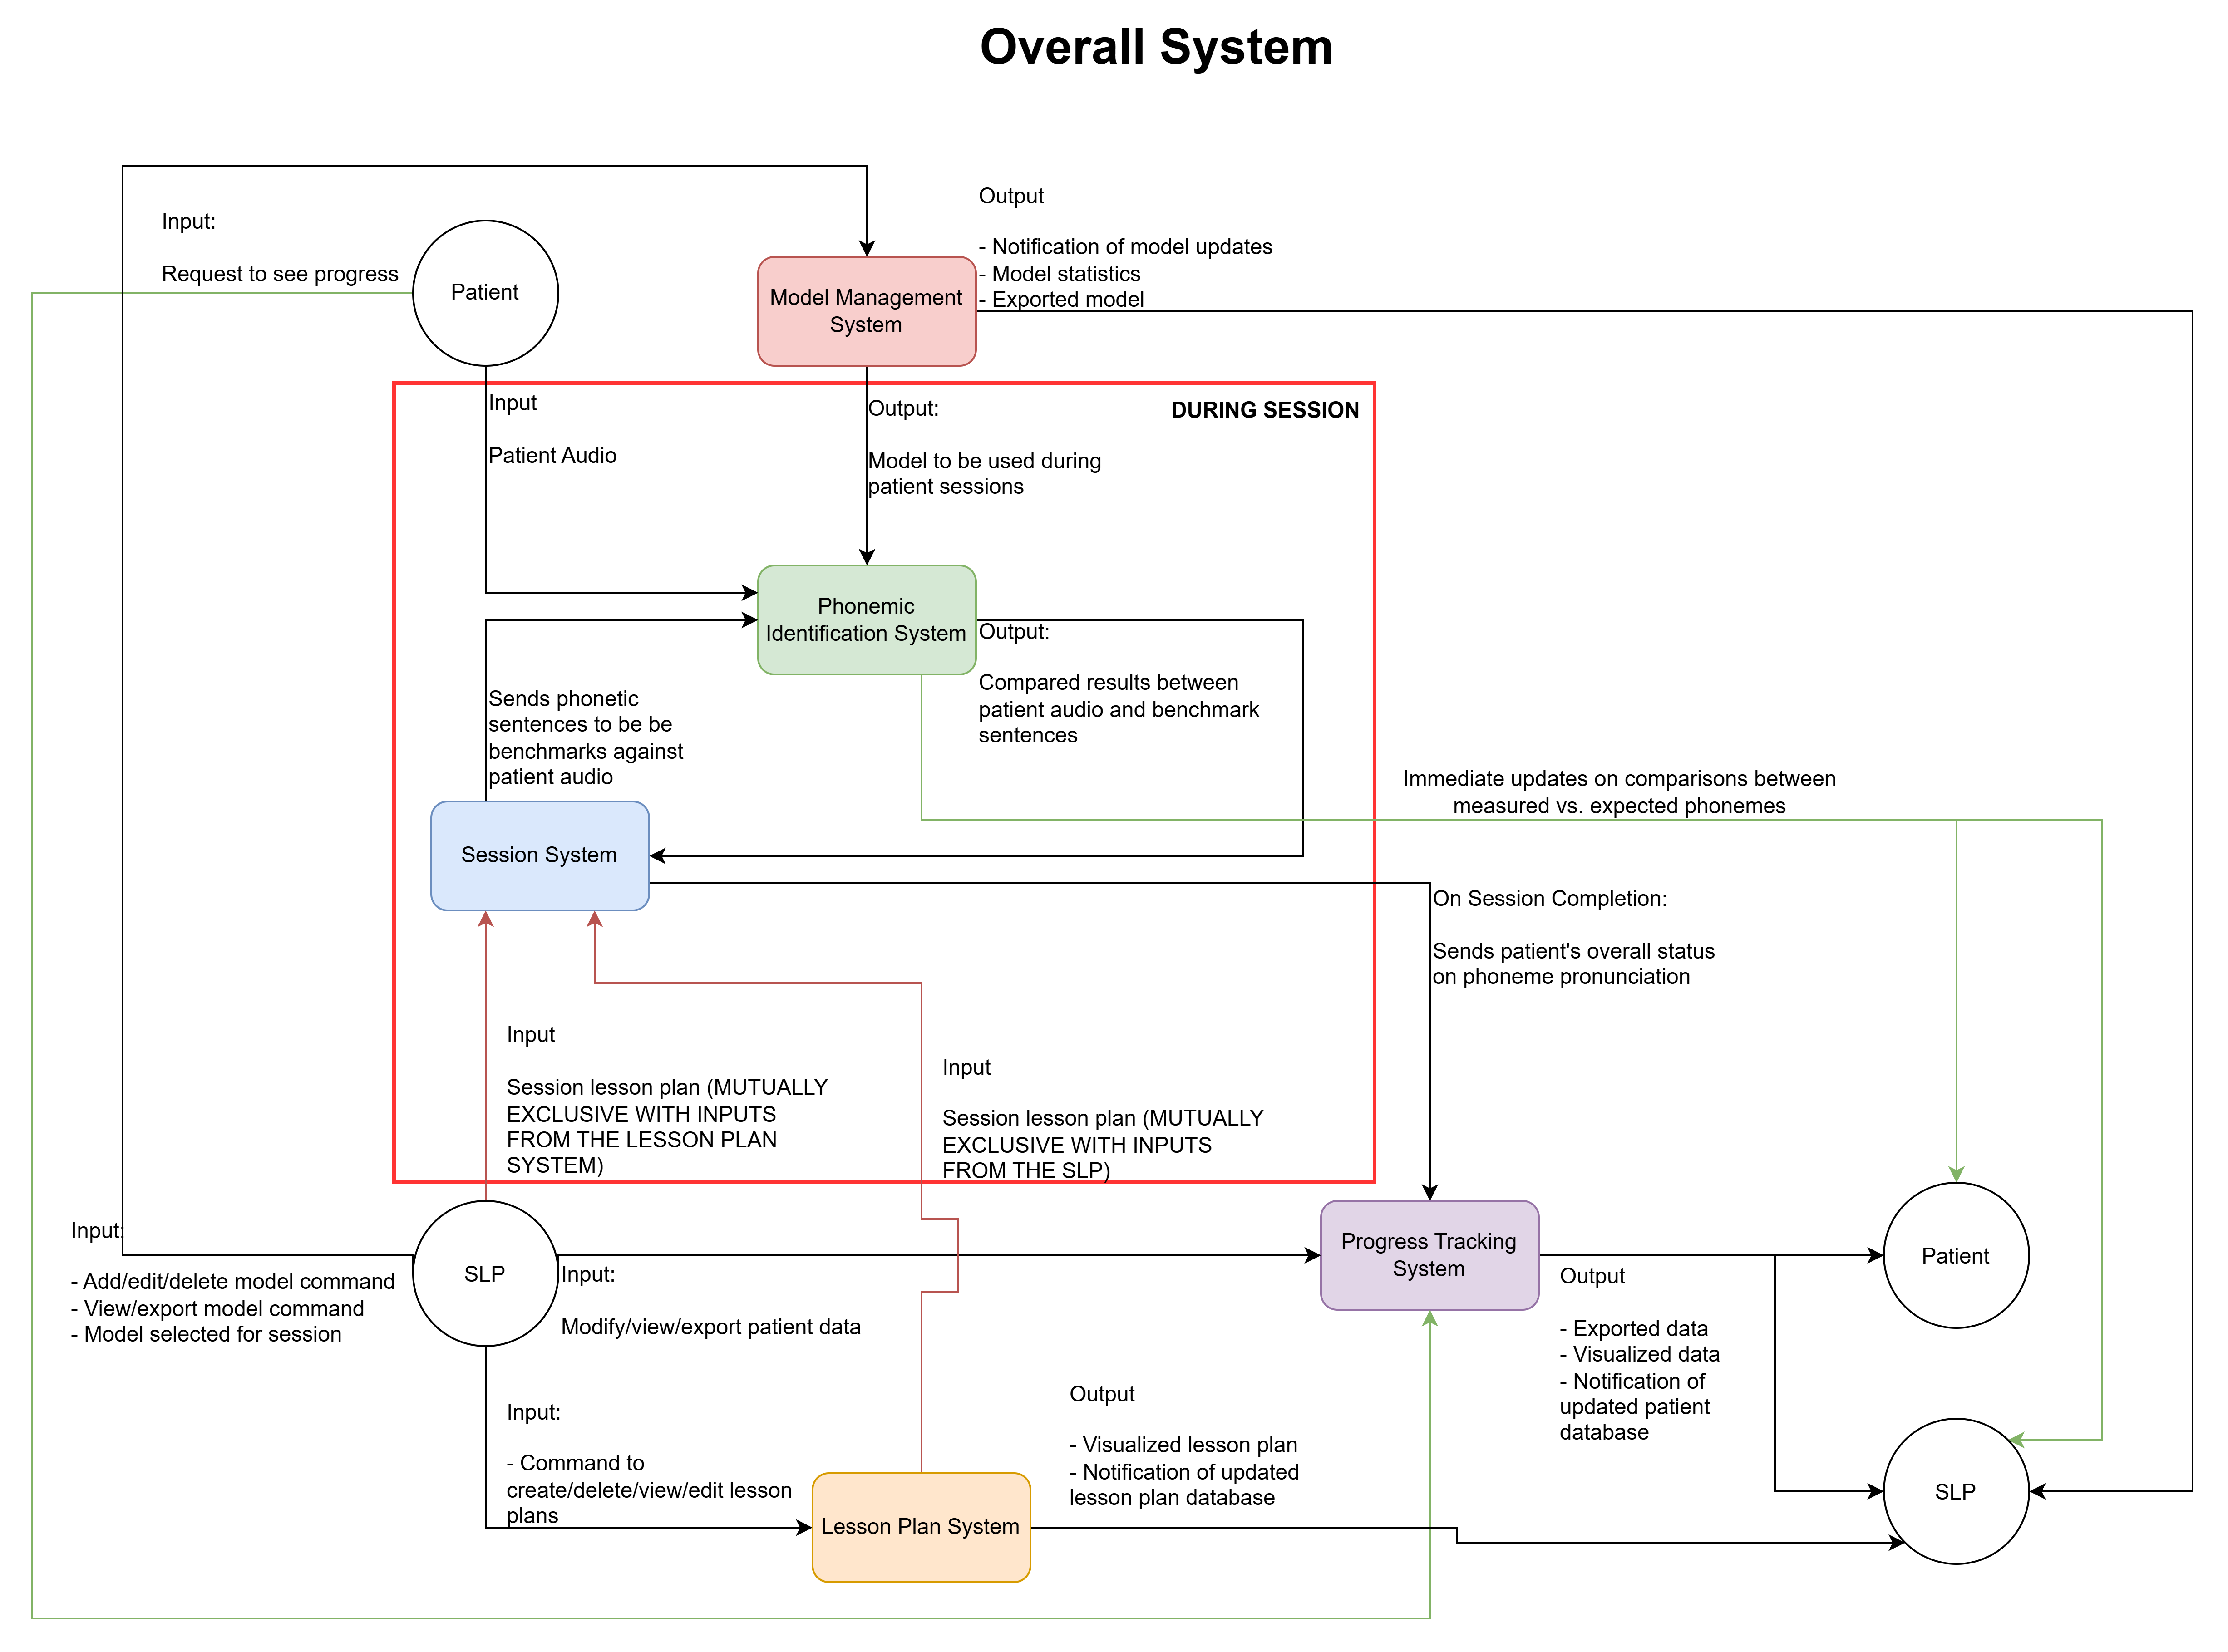
\includegraphics[width=1\linewidth]{System.png}
    \caption{Overall System Diagram}
    \label{fig:OverallSystem}
\end{figure}

\subsubsection{Patient Responsibilities}

\begin{itemize}
\item[P-R\refstepcounter{presnum}\thepresnum \label{Accuracy And Clarity}:]
When a patient is providing audio to PronouncedFish to have their speech analyzed, it is their responsibility that the audio they output is as clear as possible and as accurate to the testing phrases as they can make it
\item[P-R\refstepcounter{presnum}\thepresnum \label{Data Privacy And Sharing}:] It is up to the patient or patient’s parents/guardians that a patient is not sharing any sensitive medical data or personal information when they view their data
\end{itemize}

\subsubsection{SLP Responsibilities}

\begin{itemize}
\item[SLP-R\refstepcounter{slpresnum}\theslpresnum \label{Initiator of Sessions}:] It will be the SLP's responsibility to initiate sessions for patients. To begin a session, they will need to select the lesson plan they want to use for the session along with the phonemic identification model
\item[SLP-R\refstepcounter{slpresnum}\theslpresnum \label{Changing Patient Records}:]When an SLP makes a change to patient records, they are responsible for ensuring that the data they enter is accurate
\item[SLP-R\refstepcounter{slpresnum}\theslpresnum \label{Deleting Patient Data}:]SLPs are responsible for any patient data that they delete from the system
\item[SLP-R\refstepcounter{slpresnum}\theslpresnum \label{Changing or Adding Lesson Plans}:]When a SLP adds or changes a lesson plan, they are responsible for ensuring  the lesson plan contents are accurate to what they want to work on in a session with a patient
\item[SLP-R\refstepcounter{slpresnum}\theslpresnum \label{Deleting Lesson Plans}:]SLPs are responsible for any lesson plans they delete in the system
\item[SLP-R\refstepcounter{slpresnum}\theslpresnum \label{Patient Data Exporting}:]It is up to the SLP that whenever they export patient data for external usage, they follow PHIPA guidelines for keeping the data safe
\item[SLP-R\refstepcounter{slpresnum}\theslpresnum \label{Updates To Phonemic Identification Models}:]When an SLP wants to add or make an update a model, it is their responsibility to know where the model is sending data to ensure the system remains PHIPA compliant
\item[SLP-R\refstepcounter{slpresnum}\theslpresnum \label{Deleting Models}:] SLPs are responsible for any models they delete from the system 
\end{itemize}

\subsubsection{Context of Typical Use}

The software will typically be used in medical applications for treating patients that have speech sound disorders (SSDs). The system is neither safety-critical nor mission-critical, should the system fail, users will not be in danger and critical business/societal infrastructure will not be impacted. Since PronouncedFish is primarily an assistant to SLPs, it is not autonomously making critical medical decisions. Should the system fail during treatment, the SLP can step in with their own judgements to correct issues that come from the system. Any administrative suggestions made by PronouncedFish can be overruled by an SLPs own judgement, helping to mitigate risk for end users. 

\subsubsection{Auxilliary System Diagrams}

\begin{figure}[H]
    \centering
    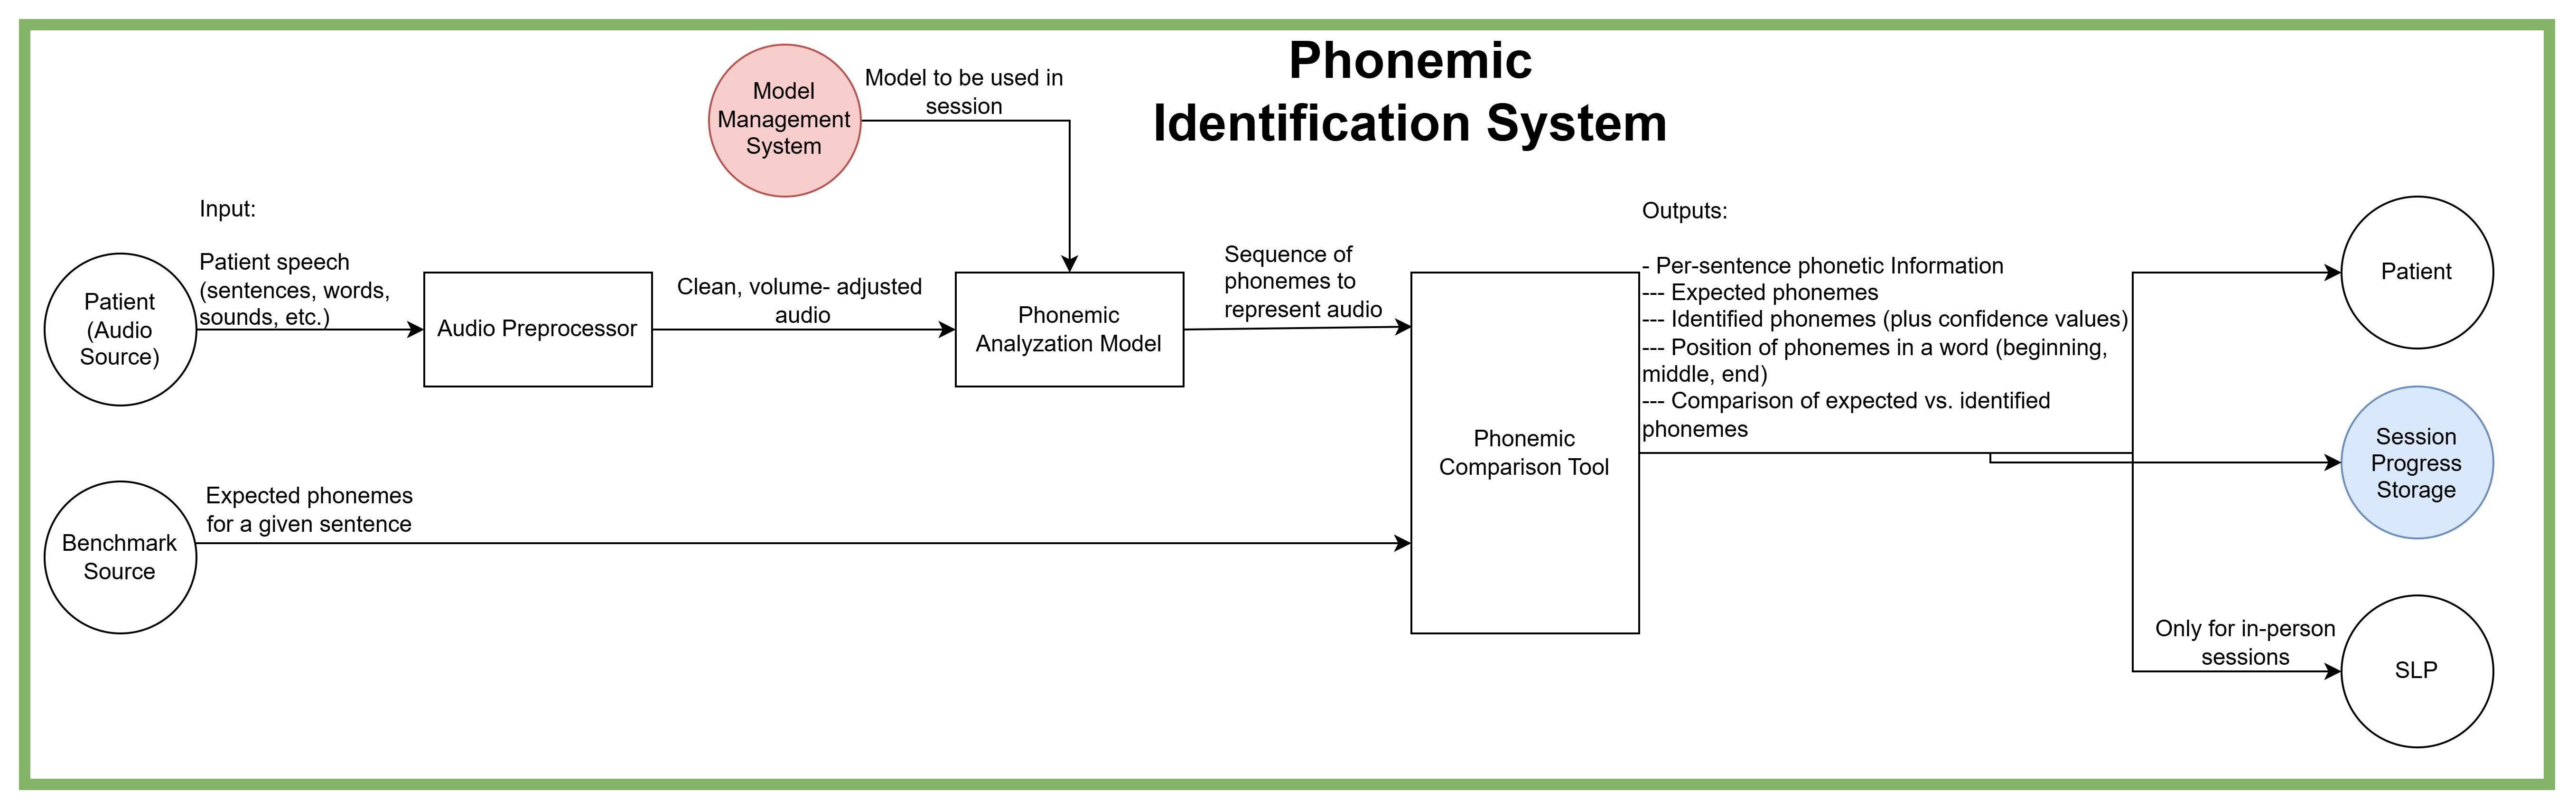
\includegraphics[width=1\linewidth]{PhonemicID.png}
    \caption{Phonemic Identification System}
    \label{fig:PID}
\end{figure}

\begin{figure}[H]
    \centering
    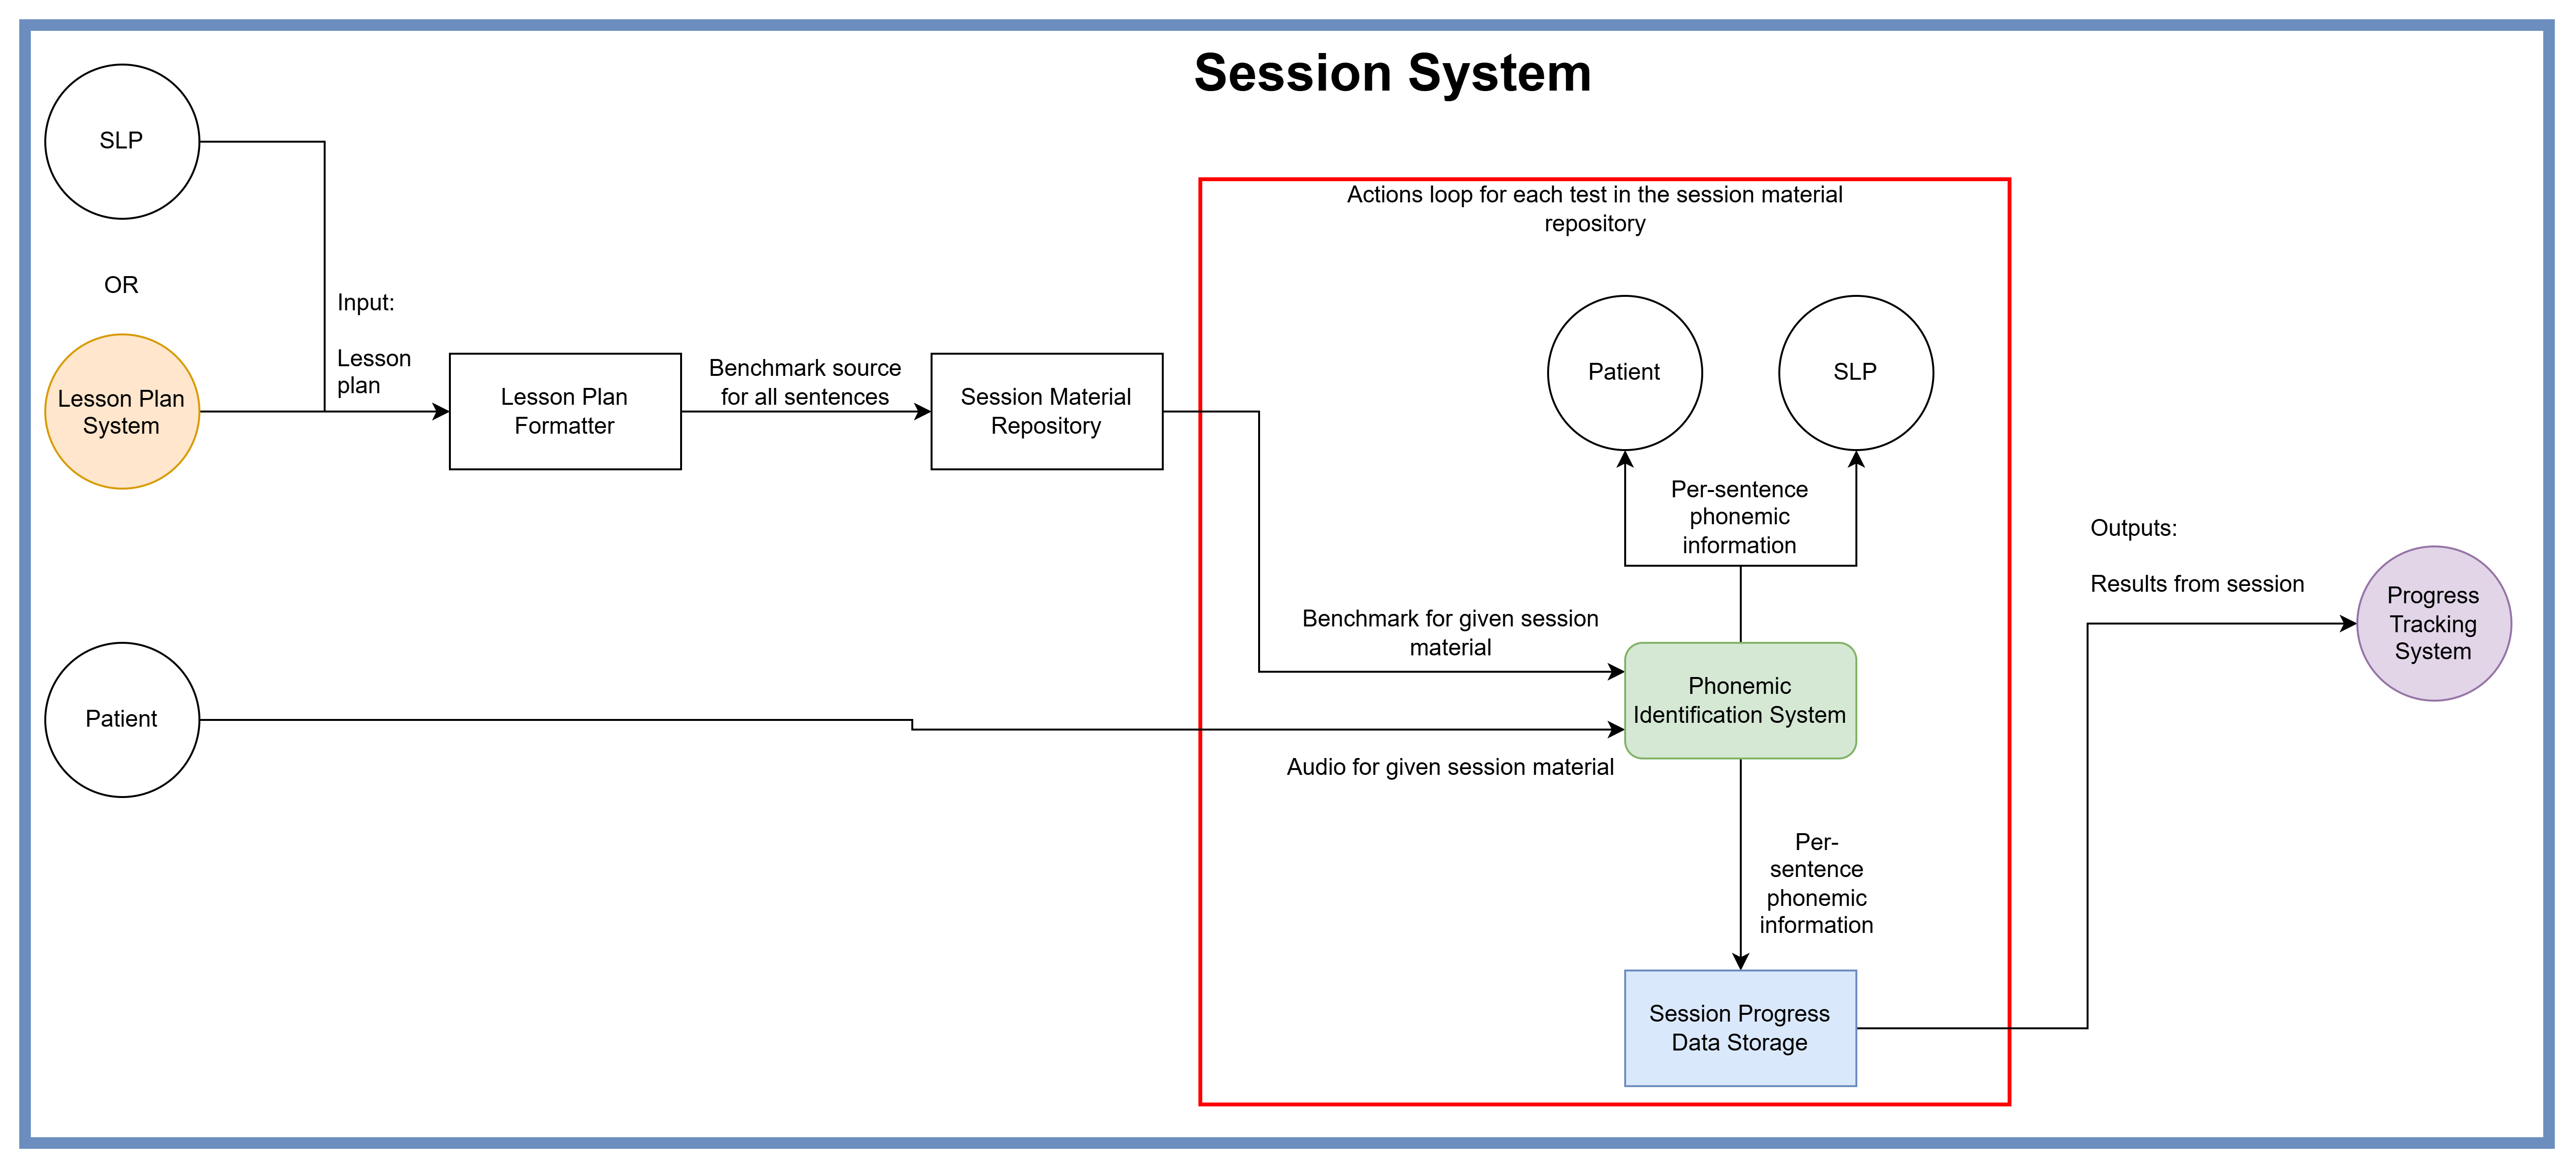
\includegraphics[width=1\linewidth]{Session.png}
    \caption{Session System}
    \label{fig:session}
\end{figure}

\begin{figure}[H]
    \centering
    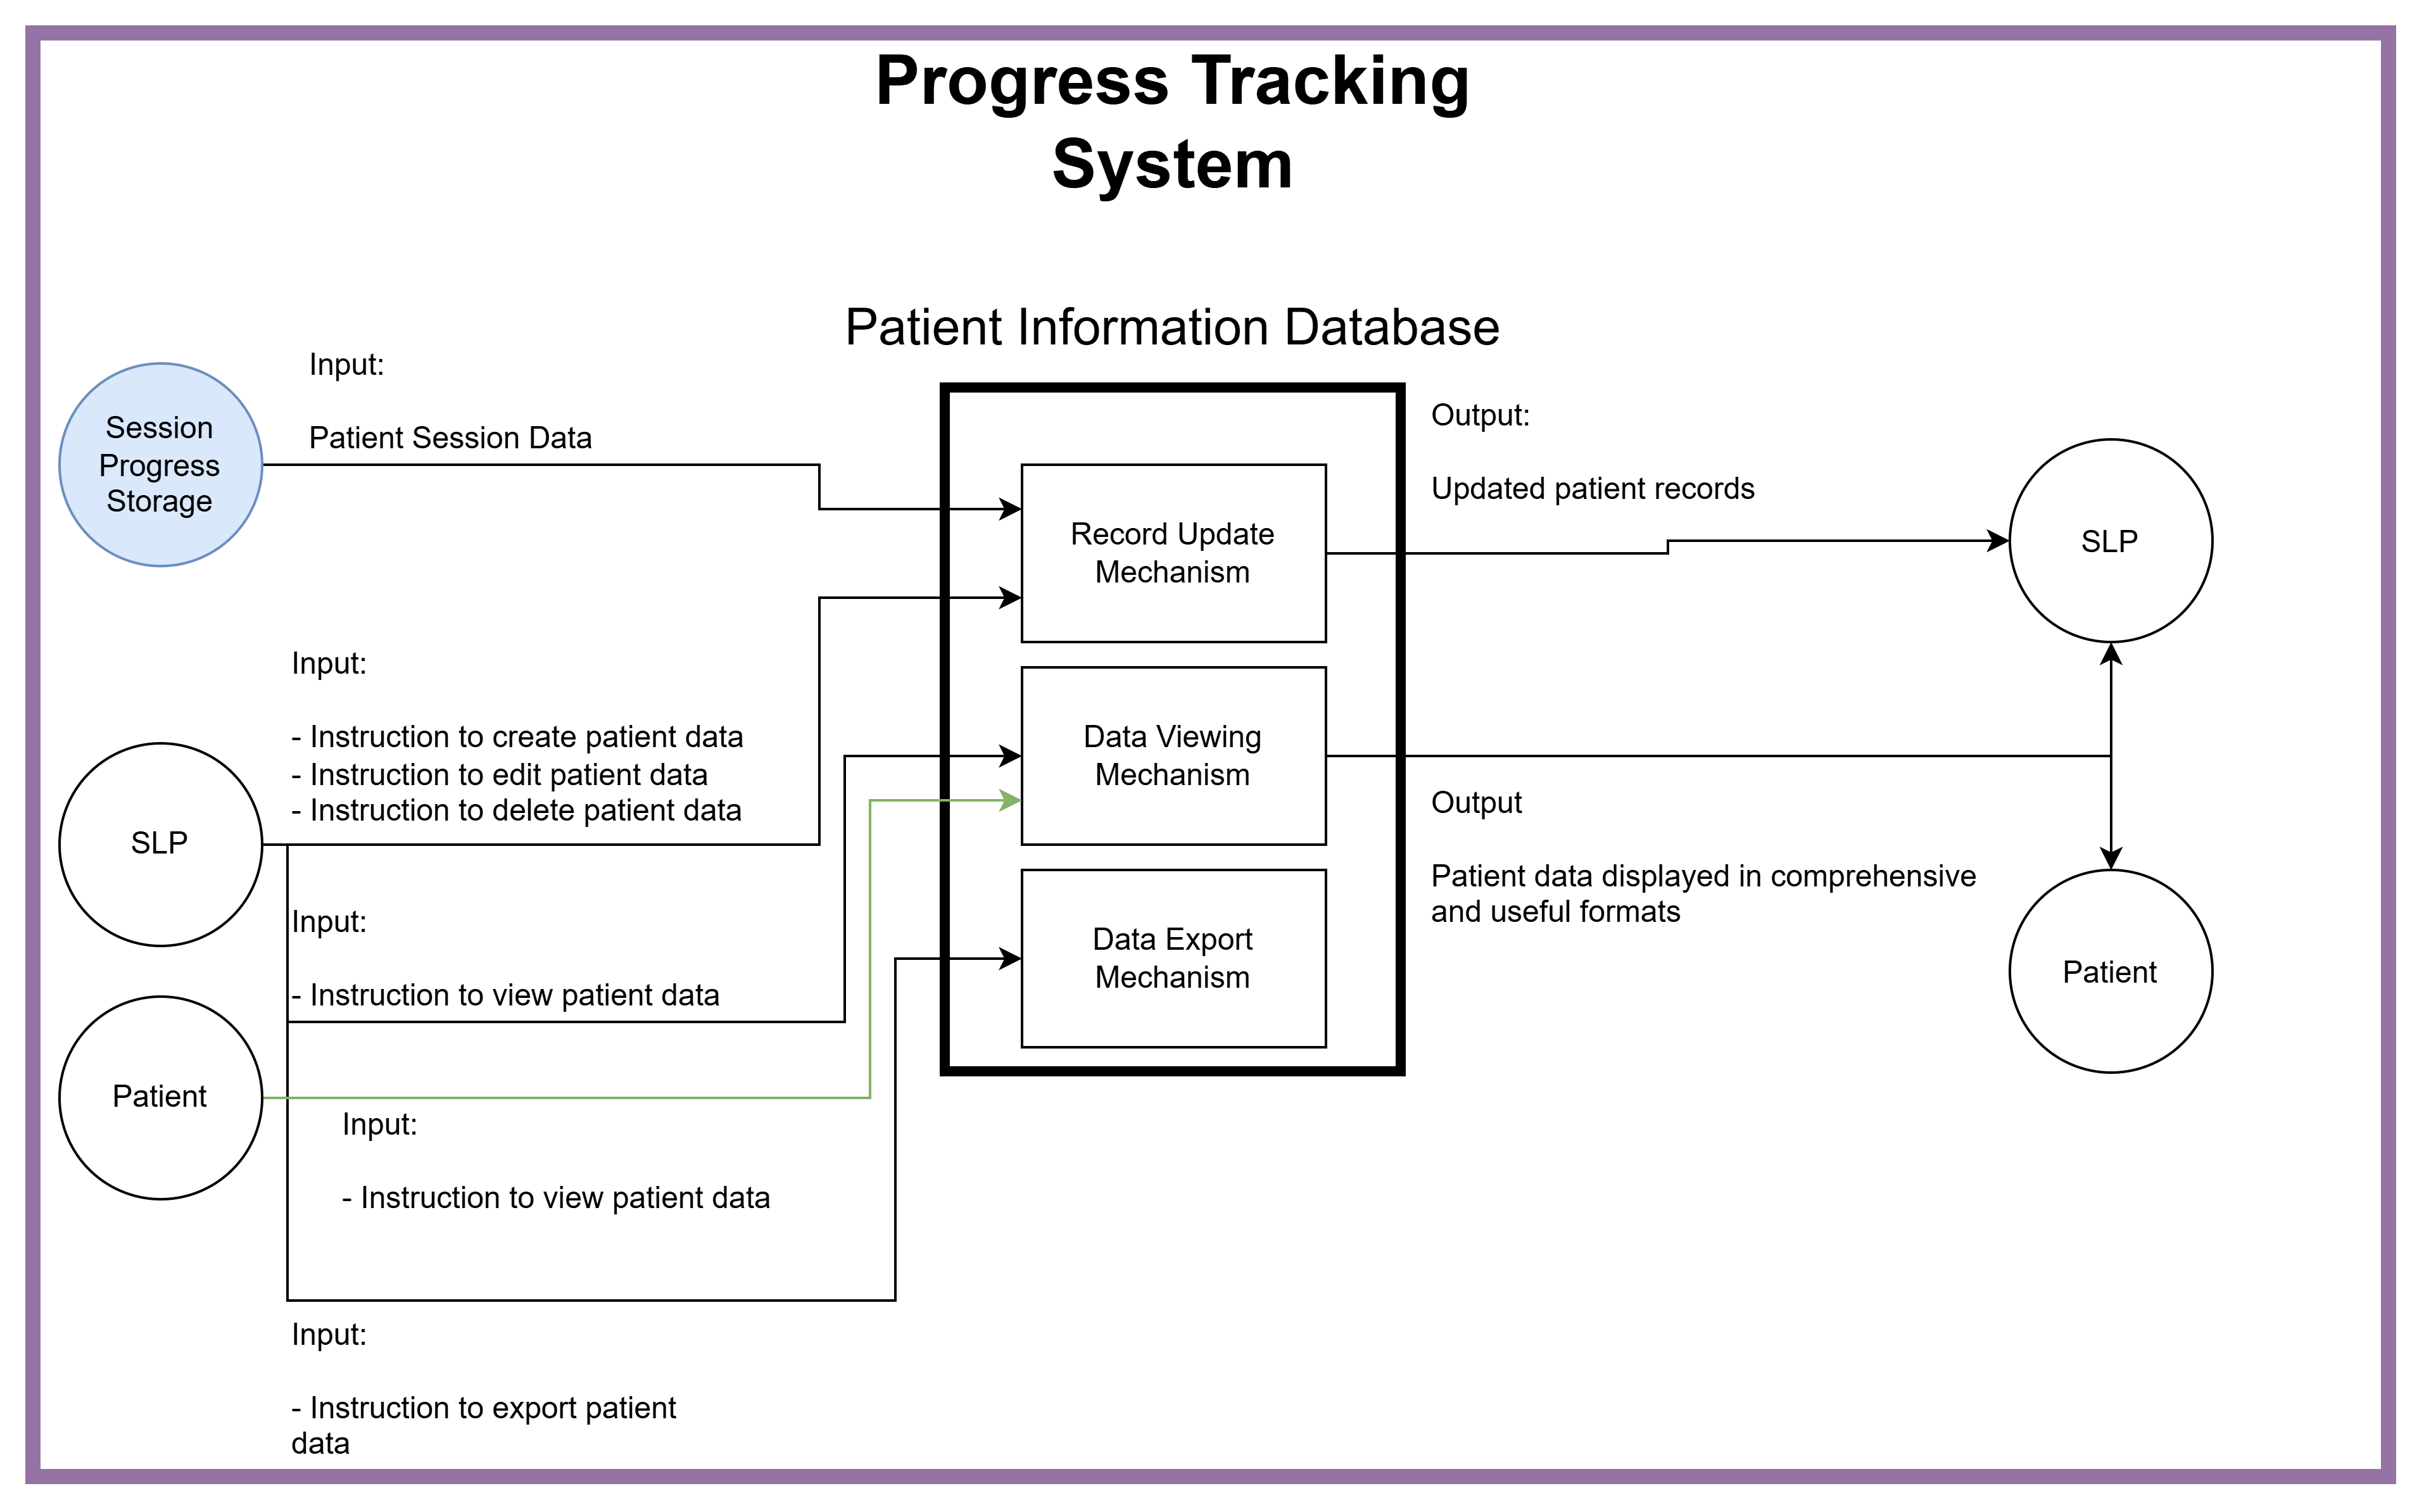
\includegraphics[width=1\linewidth]{ProgressTracking.png}
    \caption{Progress Tracking System}
    \label{fig:PT}
\end{figure}

\begin{figure}[H]
    \centering
    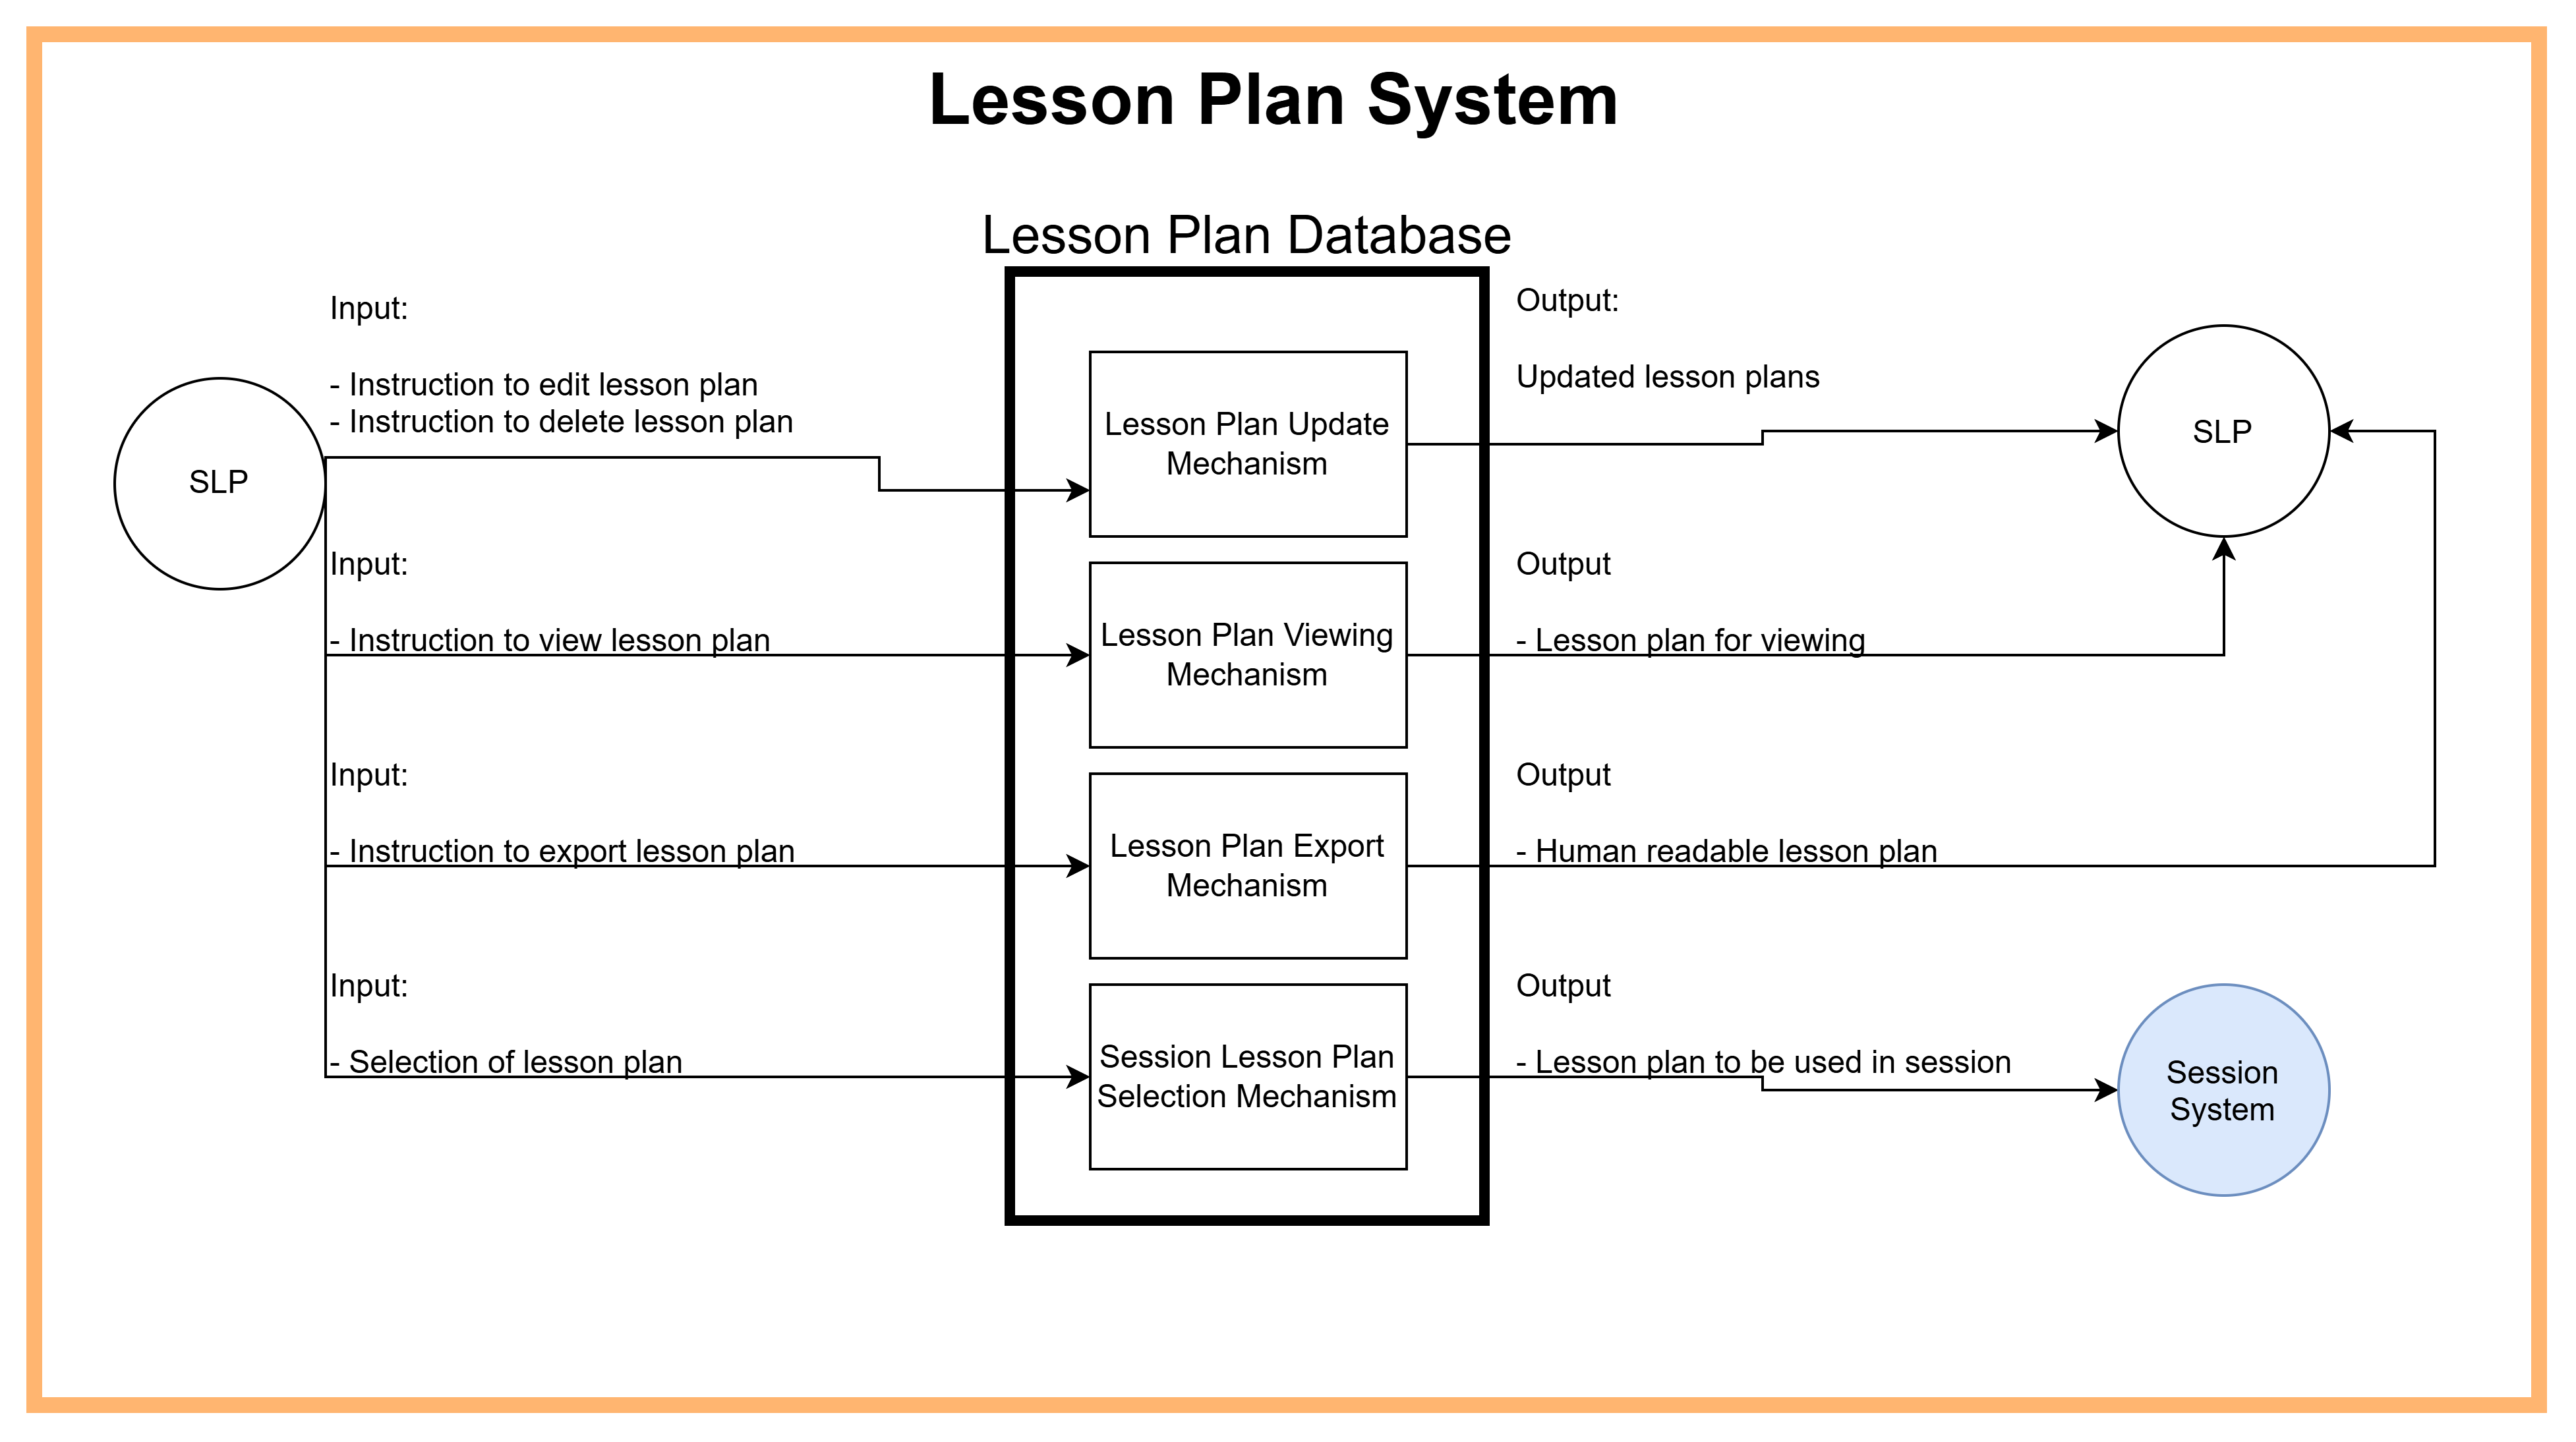
\includegraphics[width=1\linewidth]{LessonPlan.png}
    \caption{Lesson Plan System}
    \label{fig:LP}
\end{figure}

\begin{figure}[H]
    \centering
    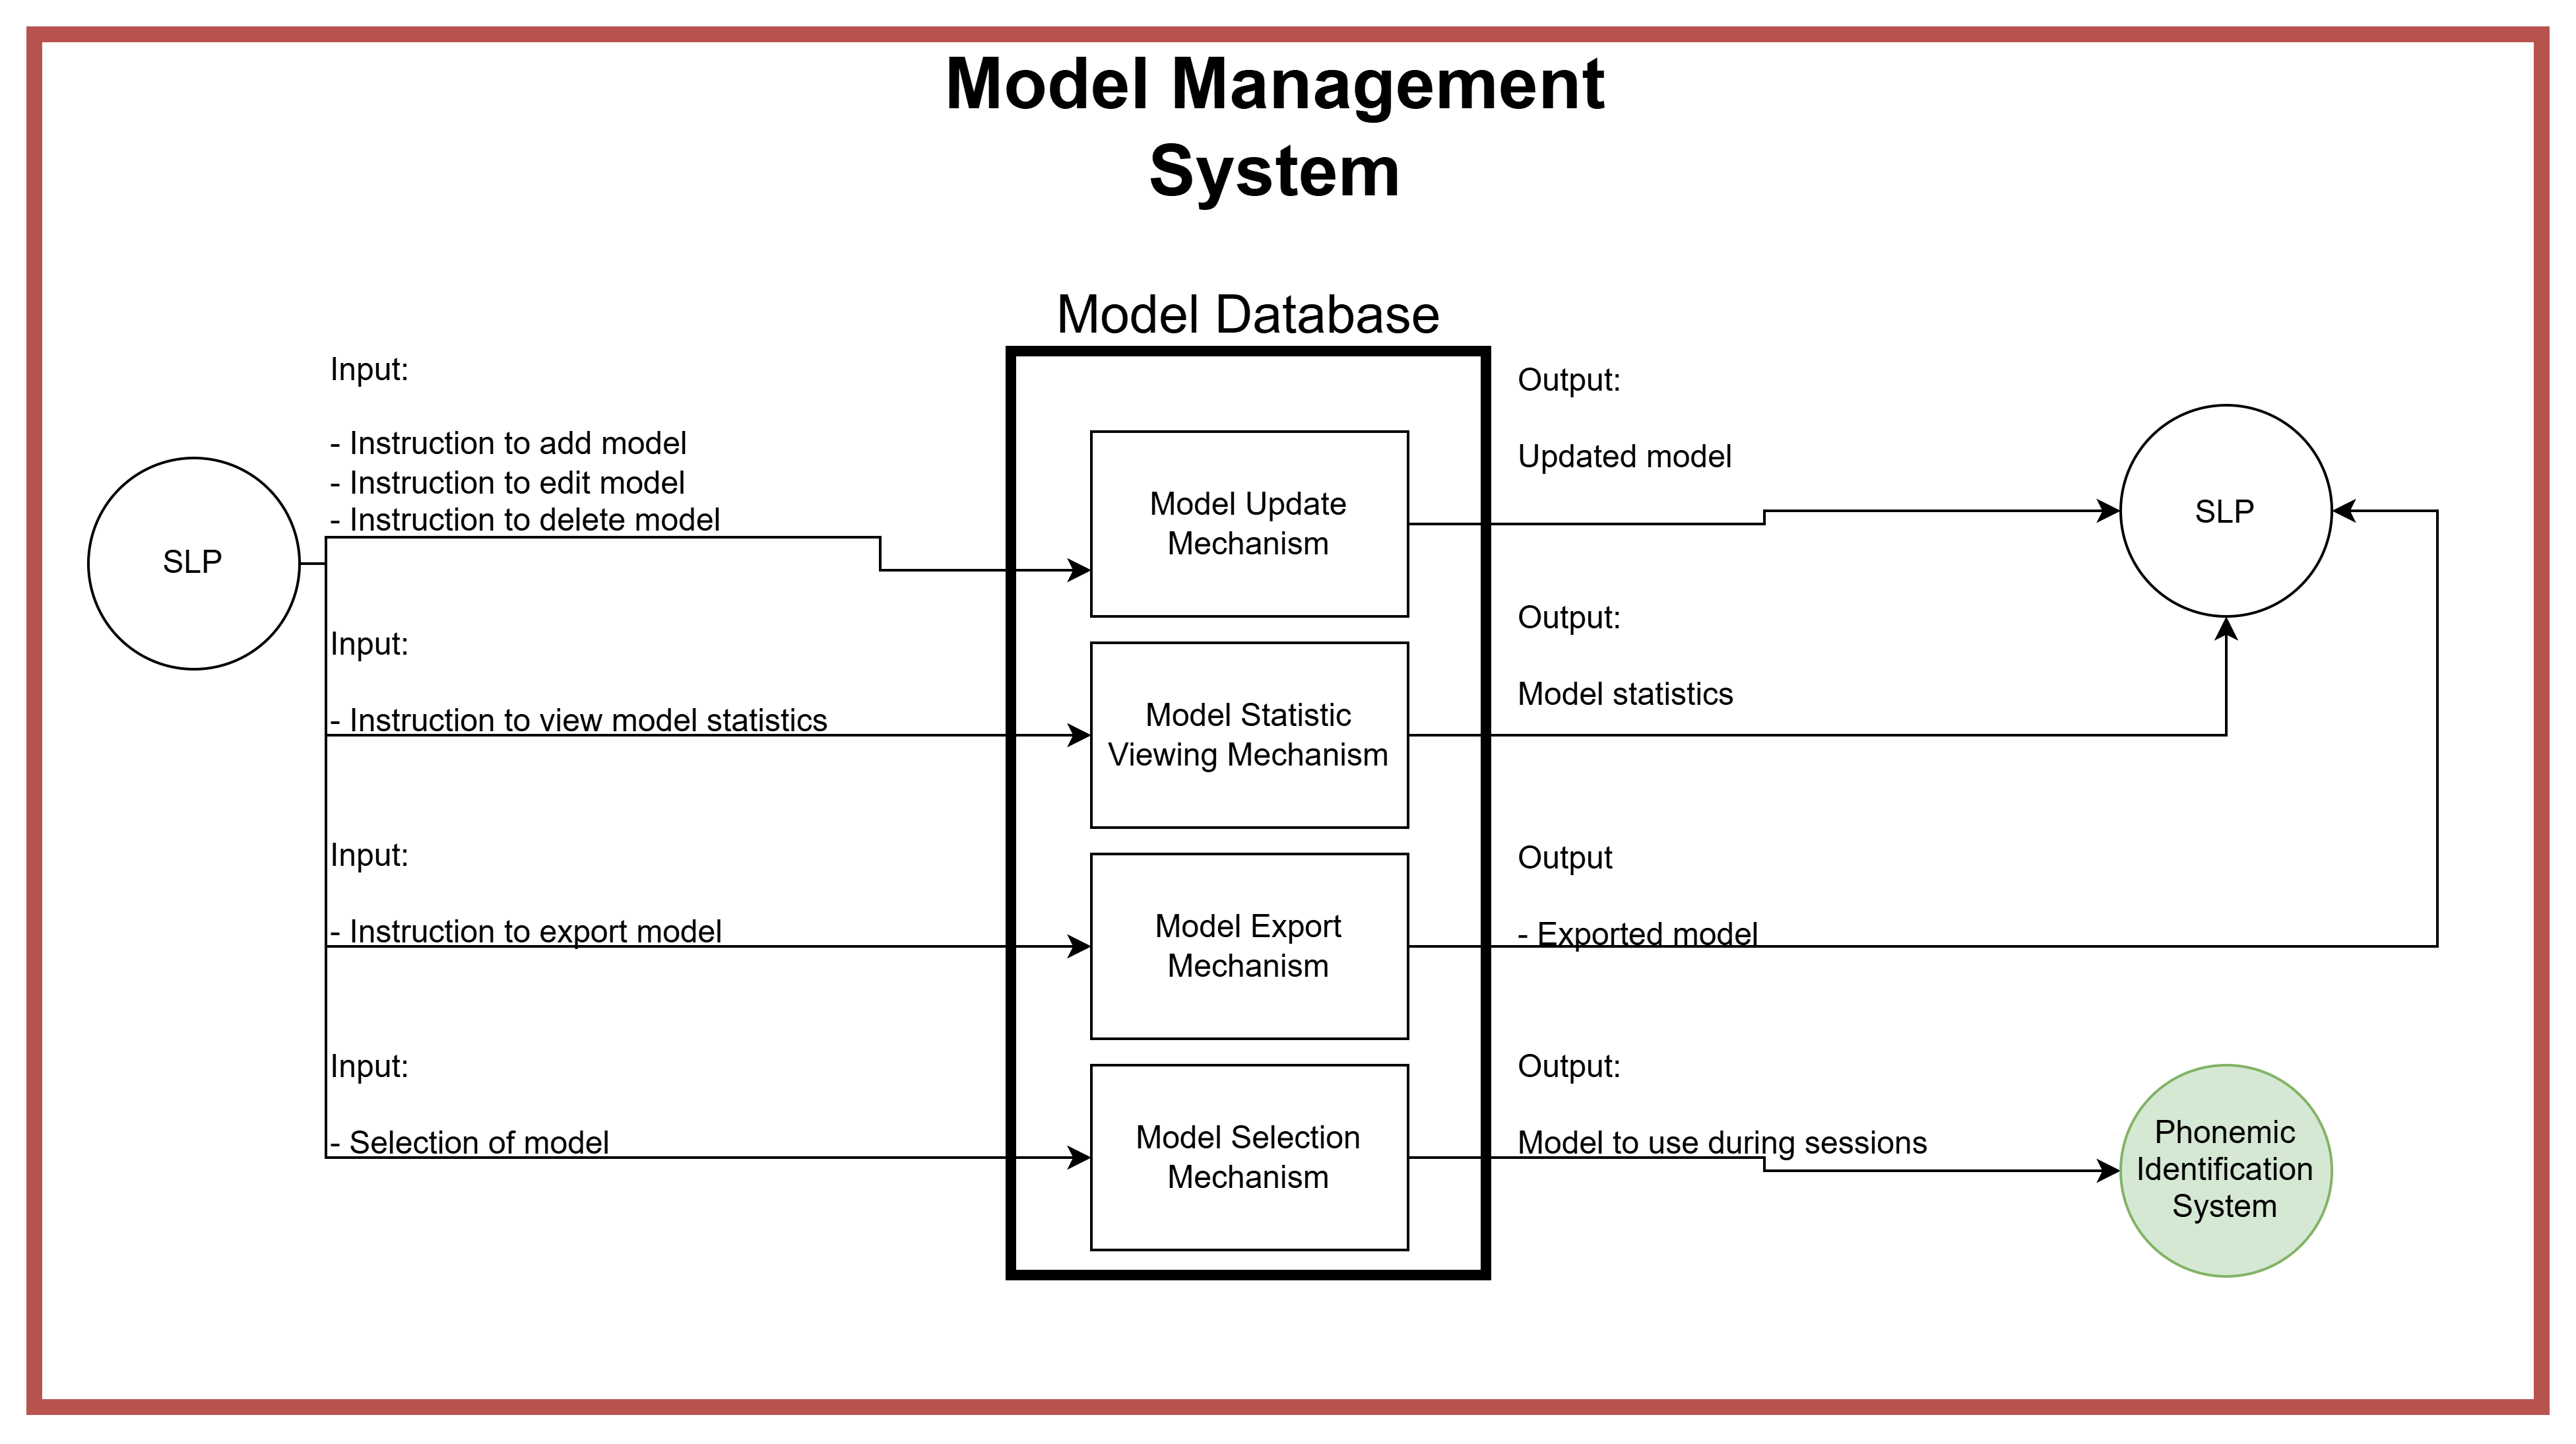
\includegraphics[width=1\linewidth]{ModelManagement.png}
    \caption{Model Management System}
    \label{fig:MM}
\end{figure}

\subsection{User Characteristics} \label{SecUserCharacteristics}

\subsubsection{Patient}
\begin{itemize}
    \item A patient is typically a child between the ages of 4-6 with an SSD like difficulties with substitutions
    \item A patient should be starting to learn how to read. PronouncedFish may use components that require a patient to read a sentence aloud. If a patient cannot read, alternative methods of treatment will be available in the system 
    \item A patient should know how repeat a sentence said by an SLP when prompted. During treatment, an SLP may ask a patient to say a sentence to get an audio sample for phonemic analysis, the patient should be able to provide such a sentence when prompted
    \item A patient will likley still be learning how to pronounce fricative phonemes (/f/, /r/, /z/) but should have an understanding of plosive phonemes (/p/, /b/, /k/, /d/) and voiced phonemes (/w/, /m/, /n/). There are still some phonemes a child has not fully learned how to say yet which will be accounted for in the system
    \item Patients have limited digital literacy, they should not need to understand the internals of how the system works to use it
    \item A patient may not be able to understand advanced data or tracking information. The data provided by PronouncedFish should readable diagrams and data tracking statistics for children above the age of 4
\end{itemize}

\subsubsection{SLP}

\begin{itemize}
    \item Expert in speech language pathology, they have a good understanding of phonemic analysis and are able to detect SSDs like substitutions.
    \item SLPs run sessions for patients, they decide which lessons to provide and which tools to use during a session to diagnose and treat SSDs. They have a good understanding of theses lessons and tools and know how to employ them effectively.  
    \item SLPs are able to track and analyze a patient's data. They are able to use data to inform them of the SSDs a patient may have an how best to treat it. They can also use the data to track the progress of treatment for a patient and use that information to guide them on which tools are best to use for future sessions.
    \item SLPs are likely not experts in machine learning, they should not need an understanding of how machine learning works to use PronouncedFish. 
    \item SLPs can use their judgements to formulate new lesson plans that are well tuned to a patients specicfic needs. 
\end{itemize}


\subsection{System Constraints}

\begin{itemize}
\item[\stepcounter{scnum}\scthescnum \label{iPad Functionality}: ]PronouncedFish and all of its functionalities must be able to run on an iPad or other kinds of tablets. \\
\textbf{Rationale: }Tablets are the most common tool for SLPs to use in a session. PronouncedFish must be able to run on existing SLP hardware to minimize the cost and training required for SLPs to be able to use the app.  
\item[\stepcounter{scnum}\scthescnum \label{Quiet Environment Constraint}: ]PronouncedFish cannot function in noisy environments.\\
\textbf{Rationale: }The system will have a more difficult time isolating a patient's voice in an environment that is noisy. At a certain level of noise, the patient's voice is indistinguishable from the surrounding noise and the app will not be able to identify phonemes.
\item[\stepcounter{scnum}\scthescnum \label{Internet Access for Authentication}: ] The system will need access the internet for authenticating a user account. \\
\textbf{Rationale: } SLPs will have accounts that they can use to access patient data, authentication of these accounts will need to happen through external services over the internet as it is infeasible to create a locally hosted authentication system.
\end{itemize}

\section{Specific System Description}

\subsection{Problem Description} \label{Sec_pd}

PronouncedFish is intended to solve the problem of identifying speech sound errors in young children during speech therapy sessions. 
Around 440,000 Canadians live with a speech, language, or communication disorder \cite{cdac2026statistics}, 
including 7-10\% of preschool children \cite{gaines2006earlyid}. 
There are several types of speech sound errors that sessions with an SLP can help with. Identifying errors, and tracking whether 
they improve over time, is a core part of an SLP's work with a patient.

Current speech analysis tools that support SLPs are limited. According to the project supervisors, some tools do not perform 
well with both speed and accuracy, especially on children's voices. Additionally, current tools and models are not tailored to 
provide real-time and interpretable analysis to an SLP during a speech therapy session. 

\subsubsection{Physical System Description} \label{sec_phySystDescrip}

PronouncedFish is a software system, but it is used within a physical setting. The physical setting for the software is a pediatric 
speech therapy session run by an SLP. 
The elements of the system's setting are described below.

\begin{itemize}

\item[PS1:] The SLP
\item Runs and supervises the therapy session.
\item[PS2:] The patient (children aged 4-6) 
\item Attends the therapy session, receiving cues and direction from the SLP, using the aid provided by PronouncedFish.
\item[PS3:] Clinic computer and technology
\item Runs the PronouncedFish software, takes input from the SLP and patient.

\end{itemize}

\begin{figure}[h!]
\begin{center}
\rotatebox{0}
{
  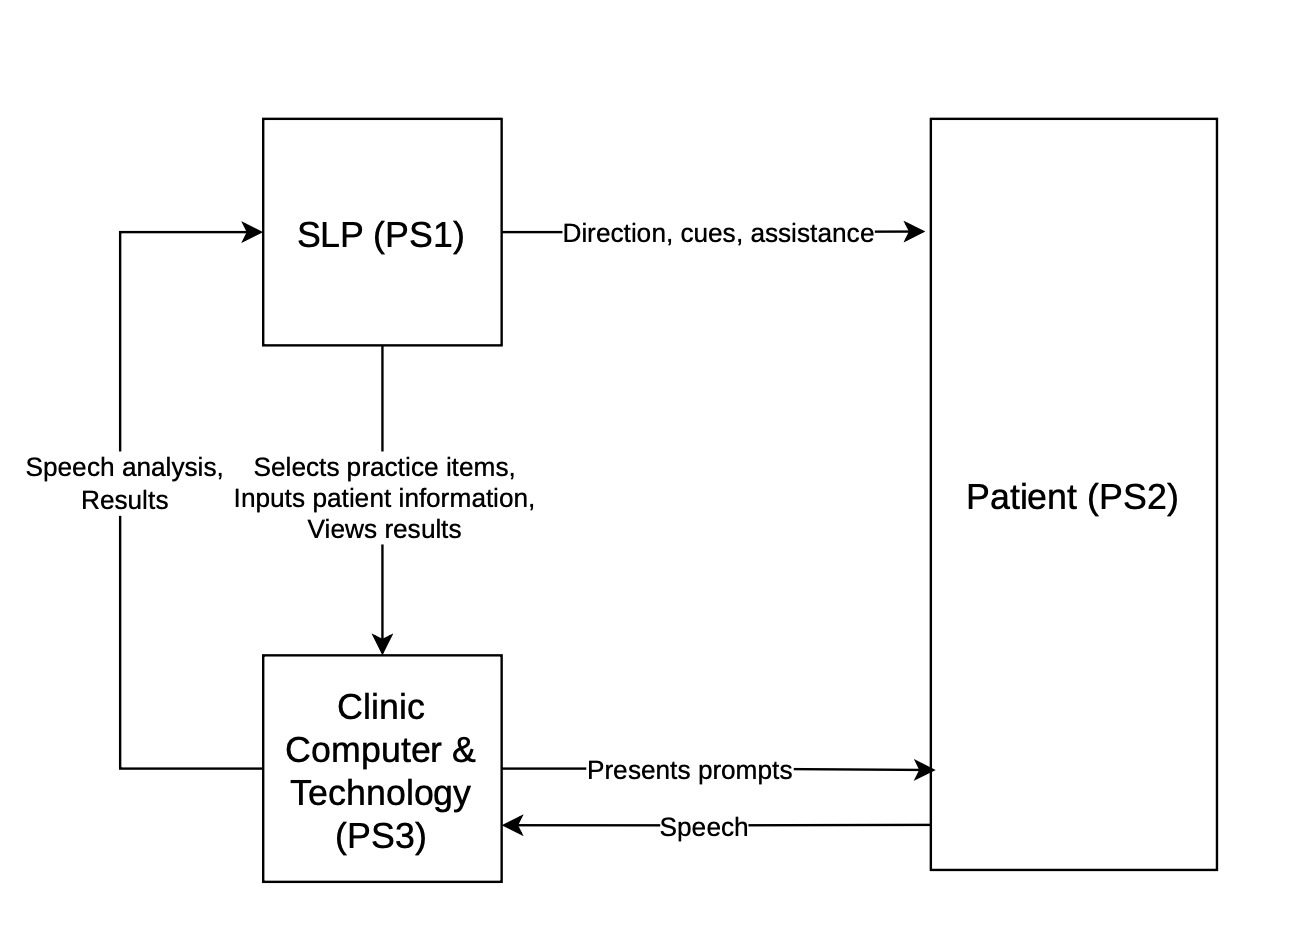
\includegraphics[width=0.5\textwidth]{GhotiPSD.png}
}
\caption{\label{<Label>} Physical System Description}
\end{center}
\end{figure}

\subsubsection{Goal Statements}

\noindent A detailed list of \href{https://github.com/lilyporter/Ghoti/blob/main/pdfs/ProblemStatementAndGoals/ProblemStatement.pdf}{Problem Statement and Goals} may be found here. For PronoucedFish, the goal statements are:

\begin{itemize}

\item \textbf{GS1}: Identify the substitution errors in a child's production of a practice item.
\item \textbf{GS2}: Present the SLP with the results, including how the produced sounds differ from the expected sounds.
\item \textbf{GS3}: Track a patient's performance on target sounds across sessions.
\item \textbf{GS4}: Support the SLP in conducting practice with the child (prompts, item selection).

\end{itemize}

\subsubsection{Scope Decisions}

The following decisions are made to narrow down the scope of the project:

\begin{itemize}
    \item \textbf{SD1}: The target demographic will be children aged 4-6.\\
    \textbf{Rationale:} A child’s phonemic inventory (the sounds they are able to speak) typically stabilizes by ages 4-6 \cite{kid_sense_dev}. If a child has speech development issues at this point, they are referred to an SLP, making this a logical age range to choose. There is a lot more variation in speech at younger ages which may be normal, so younger age ranges are unrealistic to analyze for a capstone.

    \item \textbf{SD2}: The children will be monolingual speakers with a North-American accent.\\
    \textbf{Rationale:} Speech recognition tools struggle with recognizing mistakes in bilingual people or with accented speech \cite{bias_accented_speech}. These speakers incorrectly get flagged as having speech disorders more often due to a lack of training data available for them \cite{bias_accented_speech}. This means a general all-encompassing speech analysis model is unrealistic, and the project must focus on a space with sufficient training data to work from.

    \item \textbf{SD3}: The detected speech errors will be limited to consonant substitution errors.\\
    \textbf{Rationale:} There are four main types of speech errors as per the SODA framework, and addressing them all is a significant task. For this capstone, the main issues targeted are consonant substitution errors as they are the most common \cite{common_speech_errors} and are unaffected by dialects, accents, and ways of speaking. This makes them feasible to target.

    \item \textbf{SD4}: Supported devices will be limited to iPadOS, AndroidOS, Windows desktops, and Macs.\\
    \textbf{Rationale:} When eliciting requirements with SLPs, the majority of them stated to use iPads to supplement their sessions. It is unrealistic to develop a native application for each and every operating system within the capstone timeline, so the most common platforms will be picked.
\end{itemize}

\subsubsection{Assumptions}

\begin{itemize}
\item \textbf{A1: Single-word attempts.} Each attempt consists of a single spoken target word.
\item \textbf{A2: Speaker population.} Each speaker is a monolingual North American English-speaking child aged 4--6.
\item \textbf{A3: Expected phoneme sequence.} Each target word is drawn from a standardized word set and has a predefined expected phoneme sequence $T = (t_1, \ldots, t_n)$.
\item \textbf{A4: Acceptable pronunciation variants.} Each target word has a finite, predefined set of acceptable phoneme variants $V_i$ at each position $i$, where $t_i \in V_i$.
  \begin{itemize}
  \item These sets are established in consultation with an SLP advisor to account for acceptable pronunciation variation.
  \end{itemize}
\item \textbf{A5: Substitution errors.} Each substitution error involves replacing exactly one expected phoneme with a different phoneme at the same position.
\item \textbf{A6: Sequence length mismatch.} Any difference between the recognized phoneme sequence length and the expected length $n$ is assumed to indicate at least one omission or addition.
\item \textbf{A7: SLP supervision.} Each session is conducted under the direct supervision of an SLP.
\item \textbf{A8: Unintentional pronunciation errors.} All pronunciation errors made by the speaker are assumed to be unintentional.
\item \textbf{A9: Recording conditions.} Each recording contains speech from only one speaker and is captured in a quiet environment with minimal background noise.
\item \textbf{A10: Calibrated phoneme confidence.} The recognizer's per-phoneme posterior probabilities are assumed to be calibrated, such that predicted confidence values correspond to observed frequencies of correct recognition.
\item \textbf{A11: Session devices.} SLPs are assumed to conduct sessions using an iPad, Android tablet, or computer equipped with a microphone and a modern web browser.
\end{itemize}

\subsubsection{Theoretical Models}

\begin{itemize}
\item \textbf{TM1: Phoneme recognition.} $R(x) = (P, \mathbf{c})$, where $x$ is the recorded audio, $P = (p_1, \ldots, p_m)$ is the recognized phoneme sequence, and $\mathbf{c} = (c_1, \ldots, c_m)$ are per-phoneme posteriors with $c_j \in [0, 1]$.
  \begin{itemize}
  \item Abstract mapping from audio to phonemes with confidence.
  \end{itemize}
\item \textbf{TM2: Phoneme sequence comparison.} Given $T$ (expected) and $P$ (recognized) with $|P| = n$, pair $t_i$ with $p_i$ for $i = 1, \ldots, n$.
  \begin{itemize}
  \item Positional comparison is sufficient for substitutions, which are the only errors in scope.
  \end{itemize}
\end{itemize}

\subsubsection{General Definitions}

\begin{itemize}
\item \textbf{GD1: Substitution at position $i$.} $s_i = 1$ if $p_i \notin V_i$ and $(t_i \rightarrow p_i) \in L$, otherwise $s_i = 0$, where $L$ is the predetermined list of substitution errors.
\end{itemize}

\subsubsection{Data Definitions}

\begin{itemize}
\item \textbf{DD1: Word position.} $\mathrm{pos}(i)$ is \textit{beginning} if $i = 1$; \textit{end} if $i = n$; otherwise \textit{middle}.
  \begin{itemize}
  \item Used to report where in the word each substitution occurs.
  \end{itemize}
\end{itemize}

\section{Requirements}

This section provides the functional requirements, the business tasks that the
software is expected to complete, and the nonfunctional requirements, the
qualities that the software is expected to exhibit.

\subsection{Functional Requirements}

\subsubsection{Audio Capture Requirements}

\noindent\begin{itemize}
\item \textbf{FR-AC1:} The system shall capture the patient's spoken response as audio for each attempt. \\\textbf{Rationale:} Every analysis result is derived from the recording of an attempt.
\item \textbf{FR-AC2:} The system shall use captured audio only to analyze the attempt it was captured for. \\\textbf{Rationale:} The system is scoped to data analysis only. Limiting the use of children's audio reduces privacy exposure under PHIPA.
\item \textbf{FR-AC3:} The system shall flag to the SLP any recording that fails the usability limits (noise, clipping, duration). \\\textbf{Rationale:} Noisy or malformed audio is a main cause of misclassification, so the SLP must know when a result may be unreliable.
\end{itemize}

\subsubsection{Session Management Requirements}

\begin{itemize}
\item \textbf{FR-SM1:} The system shall allow the SLP to set up a session by selecting a patient, one or more target phonemes, and target items. \\\textbf{Rationale:} Target phonemes and items define what is practised and what the analysis compares against. Selectable phonemes are limited to those covered by the predetermined substitution list (FR-SA1).
\item \textbf{FR-SM2:} The system shall allow the SLP to start, repeat, skip and end each attempt, and to end the session. \\\textbf{Rationale:} The SLP supervises the session and controls its pace.
\item \textbf{FR-SM3:} The system shall allow the SLP to record, for each attempt, whether the target was produced independently, after a semantic cue, or after repetition. \\\textbf{Rationale:} The amount of support a patient needs is a clinical indicator of progress and is tracked across sessions.
\item \textbf{FR-SM4:} The system shall allow the SLP to override the system's classification of any attempt. \\\textbf{Rationale:} The system's output is assistive and not diagnostic, so the SLP's clinical judgement takes precedence.
\end{itemize}

\subsubsection{Speech Analysis Requirements}

\begin{itemize}
\item \textbf{FR-SA1:} The system shall identify, from the captured audio of each attempt, substitutions from a predetermined list of common substitution errors, reporting the expected phoneme, the produced phoneme, and the word position. \\\textbf{Rationale:} Substitutions are the only error type in scope for the proof of concept, and accuracy is only validated for the listed errors. Word position supports the position-based visualization.
\item \textbf{FR-SA2:} The system shall not identify a substitution when the produced phoneme matches any acceptable variant defined for the target item. \\\textbf{Rationale:} Accepted North American English pronunciation varies by dialect, and treating those variants as errors would produce false substitutions.
\item \textbf{FR-SA3:} The system shall report a confidence value with each result and shall classify an attempt as ``unclassifiable'' when confidence is below the confidence threshold determined by the validation study. \\\textbf{Rationale:} The SLP can weigh uncertain results, and the system avoids forcing a classification on poor input, which reduces over-reliance on the tool.
\end{itemize}

\subsubsection{Results \& Data Visualization Requirements}
\begin {itemize}
\item \textbf{FR-RDV1:} For each speech practise attempt (word or phrase), the system shall present the expected phonemes and the phonemes it recognized to the SLP. \\
\textbf{Rationale:} The system must present this data side by side so the SLP can compare and draw conclusions from them. 
\item \textbf{FR-RDV2:} All substitution errors identified shall be displayed and indicate which expected phoneme was replaced by which produced phoneme. \\
\textbf{Rationale:} The SLP must be informed of any errors and where they occured.
\item \textbf{FR-RDV3:} The system shall include a visualization indicating the word position (beginning, middle, end) for each identified substitution. \\
\textbf{Rationale:} The visualization will make it easier for SLPs, patients, and random users to interpret the speech analysis.
\item \textbf{FR-RDV4:} The system shall include a visualization of the current session that reports, for the practice items (words/phrases) attempted, the number of correct and incorrect attempts, and, for the correct attempts, how many were produced independently and how many required additional cues or help from the SLP. \\
\textbf{Rationale:} The visualization will make it easier for SLPs, patients, and random users to interpret a summary of correct, incorrect, independent, and cued attempts this session.
\item \textbf{FR-RDV5:} The system shall include a heat-map visualization, indicating how close a produced phoneme is to the expected phoneme. \\
\textbf{Rationale:} Heat map shows produced phoneme closeness to expected phoneme for easy interpretation.
\item \textbf{FR-RDV6:} The visualizations shall update as the session is completed. \\
\textbf{Rationale:} Visualizations update automatically, so they can be reviewed as soon as the session is completed.
\item \textbf{FR-RDV7:} The system shall identify and present all visualizations as assistive and not diagnostic. \\
\textbf{Rationale:} All deductions are assistive, not diagnostic. It is important to remind users so they do not try using this to replace judgments of SLPs.
\item \textbf{FR-RDV8:} The system shall not present error information in a way that discourages the patient. \\
\textbf{Rationale:} Avoids discouraging error displays to support patient confidence.
\item \textbf{FR-RDV9:} The system shall present phonemes as the appropriate IPA symbols. \\
\textbf{Rationale:} IPA is the standard language used worldwide so these symbols must be used.
\end{itemize}

\subsubsection{Progress \& Data Management Requirements}
\begin {itemize}
\item \textbf{FR-DMR1:} The system shall maintain, for each patient, a record of identifying information and session history. 
\item \textbf{FR-DMR2:} The system shall record the support level with the attempt it applies to.
\begin {itemize}
  \item \textbf{FR-DMR2.1:} The system shall allow the SLP to input, for each attempt, the level of support the child received (eg. no additional cues, semantic cue, repetition or model from the SLP).
\end{itemize}
\textbf{Rationale:} Helps the SLP track patient progress directly within the app. 
\item \textbf{FR-DMR3:} The system shall allow the SLP to correct system output if they disagree with the system's analysis/recognition.
\begin {itemize}
  \item \textbf{FR-DMR3.1:} The system shall allow the SLP to mark an attempt as correct or incorrect regardless of the system's recognised output.
\end{itemize}
\textbf{Rationale:} The SLP judgment always overrides that of the software. This tool is purely assistive and may not be right 100\% of the time. 
\item \textbf{FR-DMR4:} For every instance in which a patient's record is viewed, created, modified, exported or deleted, the system shall record the type of information involved, the date and time, the identity of the user, and the identity of the patient the information pertains to. \\
\textbf{Rationale:} Audit log records information type, date, user, and patient to ensure traceability for all events.
\item \textbf{FR-DMR5:} The system shall allow authorized users to retrieve the audit log and to provide a copy of it on request. \\
\textbf{Rationale:} Authorized users can retrieve and copy the audit log for reference.
\item \textbf{FR-DMR6:} The system shall record, for each session, the date, the SLP, the target phonemes and words, the session results, and inputs from the SLP. 
\item \textbf{FR-DMR7:} The system shall ensure that session results are associated only with the session patient. 
\item \textbf{FR-DMR8:} The system shall track each patient's performance on target phonemes over time. 
\textbf{Rationale:} Tracks each patient's target phoneme performance over time to make informed decisions about their progress and the effectiveness of therapy.
\item \textbf{FR-DMR9:} The system shall allow the SLP to compare a patient's performance between sessions. \\
\textbf{Rationale:} Allows the SLP to evaluate patient progress given their treatment.
\item \textbf{FR-DMR10:} The system shall track and identify, for each patient, target phonemes that are showing improvement and those with persistent errors. \\
\textbf{Rationale:} Identifies improving target phonemes and persistent error patterns.
\item \textbf{FR-DMR11:} The system shall record whether a correct practised item (word/phrase) required additional cues or repetition to be achieved. \\
\end{itemize}

\subsubsection{Practice Activities Requirements}
\begin {itemize}
\item \textbf{FR-PAR1:} The system shall provide a set of practise items (words or phrases), each associated with the target phoneme(s) each one exercises and the position of that phoneme in the word. \\
\textbf{Rationale:} Allows patients to participate in speech activities directly within the app.
\item \textbf{FR-PAR2:} The system shall provide at least 3 practice items for each target phoneme in each word position (eg: with 15 target phonemes -> 15* 3 word positions * 3 items = 135 practice items). \\
\textbf{Rationale:} Ensures there is sufficient practice material for patients to use. 
\item \textbf{FR-PAR3:} The system shall allow the SLP to select practice items by target phoneme and word position. \\
\textbf{Rationale:} Allows all users to filter through and pick practice problems specific to their needs. 
\item \textbf{FR-PAR4:} The practise items shall be appropriate for the supported age range (4-6) and be drawn from a standardized set of words (i.e. Goldman Fristoe). 
\item \textbf{FR-PAR5:} For each practice item, the system shall present a prompt that elicits the child to produce the item without the SLP saying first. 
\begin {itemize}
  \item \textbf{FR-PAR5.1:} Prompts shall be in the form of image cues, rather than written words. 
  \item \textbf{FR-PAR5.2:} Prompts shall be recognisable and appropriate.
\end{itemize}
\textbf{Rationale:} Presents prompts that elicit child speech without SLP modeling.
\item \textbf{FR-PAR6:} The system shall allow the SLP to move to the next item, repeat an item, skip an item, or end the practice at any time. \\
\textbf{Rationale:} Gives the SLP complete control of the session based on how they judge patient progress and needs.
\item \textbf{FR-PAR7:} The system shall include elements that keep patients engaged during practice. 
\end{itemize}


\subsection{Nonfunctional Requirements}
    \subsubsection{Accuracy Requirements}
    \begin{itemize}
        \item \textbf{NFR-ACCU1:} The accuracy of the system for identifying phonemes will be 87\% which will be measured against the analysis and judgement of one or more speech language pathologists (SLPs).\\
        \textbf{Rationale: } Many models created after 2020 for phonemic analysis are able to achieve accuracies around the 80-90\% range \cite{auto_english_pron}.    
    \end{itemize}

    \subsubsection{Performance Requirements}
    \begin{itemize}
        \item \textbf{NFR-PER1:} Phonemic estimation results must be presented in less than 10 seconds for a short sentence.\\
        \textbf{Rationale:} This is because 10 seconds is the limit for sustaining a user's attention during a human-computer dialogue before they will want to perform other tasks \cite{software_response_times}.
    \end{itemize}

    \subsubsection{Usability Requirements}
    \begin{itemize}
        \item \textbf{NFR-USA1:} The SLP must be able to fully navigate the software within one hour of use.\\
        \textbf{Rationale:} We expect that it will take some time to become accustomed to the software, but we do not want the software to be a time sink.
        \item \textbf{NFR-USA2:} The SLP cannot delete critical data without a confirmation or the ability to recover it within 72 hours.\\
        \textbf{Rationale:} This provides a safety net for the SLP to prevent accidental deletion of critical data.
        \item \textbf{NFR-USA3:} The time spent using the software tool during and outside of a session should be less than the time spent using equivalent manual tools.\\
        \textbf{Rationale:} The software is intended to improve efficiency, and any loss in efficiency would be counterproductive.
        \item \textbf{NFR-USA4:} The child cannot access the rest of the system beyond the gamified experience.\\
        \textbf{Rationale:} This provides a safety measure to ensure that the child cannot access data without the supervision of the SLP.
    \end{itemize}

    \subsubsection{Maintainability Requirements}
    \begin{itemize}
        \item \textbf{NFR-MAI1:} The software should be modular to allow extension to interfaces for other professions (e.g., accent coaches and language teachers).\\
        \textbf{Rationale:} We anticipate the value of extending the software, and a modular design facilitates this.
        \item \textbf{NFR-MAI2:} The software should be modular to allow extension to other speech differences under SODA.\\
        \textbf{Rationale:} We anticipate the value of extending the software, and a modular design facilitates this.
        \item \textbf{NFR-MAI3:} Building and deploying a patch should take less than 30 minutes.\\
        \textbf{Rationale:} This is to ensure that the software is updated in a timely manner, ideally before the next session with a child for critical bug fixes.
    \end{itemize}

    \subsubsection{Portability Requirements}
    \begin{itemize}
        \item \textbf{NFR-POR1:} The web-based application should work on Windows, macOS, iOS, and Android.\\
        \textbf{Rationale:} Although this is a web-based application, compatibility with common operating systems still needs to be ensured.
        \item \textbf{NFR-POR2:} The web-based application should work on Chrome, Firefox, Safari, and Edge browsers.\\
        \textbf{Rationale:} This covers some of the most commonly used browsers, including default browsers such as Safari on macOS and Edge on Windows.
        \item \textbf{NFR-POR3:} The web-based application should work on desktop, tablet, and laptop devices.\\
        \textbf{Rationale:} The majority of SLPs will likely use one of these devices, with iPads (tablets) being particularly common \cite{supervisor2026initialcomm}.

    \end{itemize}

    \subsubsection{Reliability Requirements}
    \begin{itemize}
        \item \textbf{NFR-REL1:} Server-side actions (login/out, data storage and retrieval) have a maximum latency of 10 seconds. \\
        \textbf{Rationale: } Should SLPs be using the program frequently, SLPs can almost always be sure any transaction they make with servers will take at most 10 seconds. 
        \item \textbf{NFR-REL2:} The system will operate at max performance from 6am to 12am. \\
        \textbf{Rationale: } Since there will be portions of PronouncedFish that are continuously operational (data storage and authentication), those systems will operate at max efficiency during the times that SLPs are most likely to conduct treatments, those times being 6am-12am.
        \item \textbf{NFR-REL3:} The system will be minimally operational between 12am to 6am outside of SLP work hours. \\
        \textbf{Rationale: } Since there will be portions of PronouncedFish that are continuously operational (data storage and authentication), there will be times where the system is not being extensively used (mainly outside of SLP work hours). During those times, the system can operate slower and consume less energy to run since the number of people using the system at that time is few to zero.
        \item \textbf{NFR-REL4:} Required maintenance, system health checkups, and system updates happen no more than every 1-2 months and during minimal operation hours \\
        \textbf{Rationale: } Possible server or data storage maintenance will be required to keep the system running and trusted. Whenever non-critical checkups/maintenance/updates need to happen, they will happen during SLP off hours so the impact on the SLPs are minimized.
    \end{itemize}

    \subsubsection{Security and Privacy:} 
    \begin{itemize}
        \item \textbf{NFR-SAP1:} The system will encrypt all PHI as it is collected using strong up-to-date encryption standards \\
        \textbf{Rationale: } To protect user information from cyber attacks, any sensitive health information that may be collected or used in treatments is immediately encrypted. This prevents attackers from reading or getting significant information on a patient.
        \item \textbf{NFR-SAP2:} The system will use a secure cryptographic protocol for communications for all data traffic between system components\\
        \textbf{Rationale: } The system may require PHI to be sent through the internet, especially for data management. This leaves it open to interception by third parties, therefore, a secure communication protocol that prevents third parties from interpreting sensitie information.
        \item \textbf{NFR-SAP3:} The system will provide outlets for SLPs to anonymize PHI that is collected from a patient. \\
        \textbf{Rationale: } Data must be able to be anonymised to remain compliant with PHIPA and prevent compromised data from being used to identify patients. 
    \end{itemize}

    \subsubsection{Legal and Licensing:} 
    \begin{itemize}
        \item \textbf{NFR-LAL1:} The system will follow the Personal Health Information Protection Act (PHIPA) guidelines for data storage, data transfer, data access and data residency.\\
        \textbf{Rationale: } SLPs are required to work within the guidelines of PHIPA to protect patient information. Thus, the tools they use in sessions must also not violate PHIPA guidelines.
        \item \textbf{NFR-LAL2:} The system will be open source using the GNU General Public License (GPL).\\
        \textbf{Rationale:} The materials that are used to make PronouncedFish are licensed under the GNU GPL. Thus, PronouncedFish itself becomes licensed under GNU GPL and becomes open source.
    \end{itemize}


\section{Likely Changes}    

Below is a list of requirements that are likely to change. The provided rationale will explain whether this is due to a scope decision, stretch goal, or other factor. 
\begin{itemize}
    \item \textbf{LC1}: The speech analysis model shall identify omission, distortion and addition phonetic articulation errors as described in the SODA framework.\\
    \textbf{Rationale:} Due to scope requirements, speech error detection has been limited to just substitution errors for this project. Ideally, this will be changed to analyze all forms of errors.\\
    \textbf{Related Assumption(s):} A5, A6

    \item \textbf{LC2}: The speech analysis model will fairly accommodate accents originating from regions outside North America. Fair implies the model will recognize errors at a comparable accuracy (+/- 5\% relative to the North American accent) for speakers of any accent.\\
    \textbf{Rationale:} Due to scope requirements, the child’s accent has been limited to just Monolingual North American speakers. English speakers are very diverse, and there must be adequate support for users from all backgrounds.\\
    \textbf{Related Assumption(s):} A2

    \item \textbf{LC3}: The system shall provide an interface for an SLP to assign homework to their patients.\\
    \textbf{Rationale:} The first iteration of the system will provide an interface for an SLP-led session in the clinic. A stretch goal is to allow patients to complete homework at home, but this is not a core feature, so it is a likely change.\\
    \textbf{Related Assumption(s):} A7

    \item \textbf{LC4}: The system shall highlight errors for children of all age ranges based on the standardized speech sound development chart.\\
    \textbf{Rationale:} Due to scope requirements, the target child age has been restricted to ages 4-6. Speech errors may occur at any age, and even for adults. Therefore, more flexibility will be crucial in future iterations of the product.\\
    \textbf{Related Assumption(s):} A2

    \item \textbf{LC5}: The system will support being locally hosted on Windows and Mac operating systems. The system will have compatible mobile apps for iOS and Android OS. The system will be supported in Safari and Google Chrome browsers.\\
    \textbf{Rationale:} SLPs may conduct their sessions using iPad, tablet, or computer microphones, so all platforms must be supported. They also deal with confidential patient health information, so web-based solutions may not be trusted.\\
    \textbf{Related Assumption(s):} A11
\end{itemize}

\section{Unlikely Changes}    

\begin{itemize}

    \item \textbf{UC1:} The system will shift its focus to working with adults instead of children.\\
    \textbf{Rationale:} The goal of PronouncedFish is to help children with SSDs in the early stages of their phoneme-pronouncing journey. Switching to working with adults will require different models for phonemic identification and different datasets to train them to be effective.
    \item \textbf{UC2:} The system will change its guidelines from PHIPA to something else.\\
    \textbf{Rationale:} Since Ontarian SLPs mostly work with PHIPA, using a different guideline would be counterproductive and unrepresentative of the target SLP user base. The guidelines should only change if new laws are enacted that supersede PHIPA.
    \item \textbf{UC3:} The system will shift its focus away from English speakers.\\
    \textbf{Rationale:} Whilst in theory possible for PronouncedFish to work with languages other than English, members of the team and the supervisors primarily work with English speaking patients, thus the models and system should be fine-tuned to work with English speakers.
    \item \textbf{UC4:} The system will use generative AI to create lesson plans.\\
    \textbf{Rationale:} SLPs are the experts when it comes to knowing what a patient needs to treat their SSDs. While this feature is possible to implement, Ghoti entrusts the responsibility of creating new lesson plans with the SLPs due to their expertise. 

\end{itemize}

\section{Traceability Matrices and Graphs}

The following traceability matrices map relationships between the various requirements and design
decisions made throughout this document. The first one traces relations between the functional 
and non-functional system requirements. The second matrix links the assumptions 
to all other goals, scope decisions, and items. Each relation is marked by an X between the corresponding items.  


% Traceability matrix 1 (i)

\clearpage
\scriptsize
\setlength{\tabcolsep}{4pt}
\renewcommand{\arraystretch}{1.15}

\begin{longtable}{|
    >{\centering\arraybackslash}p{1.6cm}|
    *{9}{>{\centering\arraybackslash}p{0.85cm}|}
}
\caption{Traceability Matrix: Functional and Nonfunctional Requirements (1)}
\label{Table:FR_NFR_trace_1}\\
\hline

\multicolumn{1}{|c|}{\multirow{2}{*}{\textbf{Functional}}} &
\multicolumn{9}{c|}{\textbf{Nonfunctional}} \\
\cline{2-10}
\multicolumn{1}{|c|}{} &
\textbf{ACU1} & \textbf{PER1} &
\textbf{USA1} & \textbf{USA2} & \textbf{USA3} & \textbf{USA4} &
\textbf{MAI1} & \textbf{MAI2} & \textbf{MAI3} \\
\hline
\endfirsthead

\multicolumn{10}{|l|}{\textit{Traceability Matrix (1), continued}}\\
\hline
\multicolumn{1}{|c|}{\multirow{2}{*}{\textbf{Functional}}} &
\multicolumn{9}{c|}{\textbf{Nonfunctional}} \\
\cline{2-10}
\multicolumn{1}{|c|}{} &
\textbf{ACU1} & \textbf{PER1} &
\textbf{USA1} & \textbf{USA2} & \textbf{USA3} & \textbf{USA4} &
\textbf{MAI1} & \textbf{MAI2} & \textbf{MAI3} \\
\hline
\endhead

\hline
\multicolumn{10}{|r|}{\textit{Continued on next page}}\\
\hline
\endfoot

\hline
\endlastfoot

AC1  & & & & & & & & & \\ \hline
AC2  & & & & & & & & & \\ \hline
AC3  & & & & & & & & & \\ \hline
SM1  & & & & & & & & & \\ \hline
SM2  & & & & & & & & & \\ \hline
SM3  & & & & & & & & & \\ \hline
SM4  & & & & & & & & & \\ \hline
SA1  & & & & & & & & & \\ \hline
SA2  & & & & & & & & & \\ \hline
SA3  & & & & & & & & & \\ \hline
RDV1 & & & & & & & & & \\ \hline
RDV2 & & & & & & & & & \\ \hline
RDV3 & & & & & & & & & \\ \hline
RDV4 & & & & & & & & & \\ \hline
RDV5 & & & & & & & & & \\ \hline
RDV6 & & & & & & & & & \\ \hline
RDV7 & & & & & & & & & \\ \hline
RDV8 & & & & & & & & & \\ \hline
RDV9 & & & & & & & & & \\ \hline
DMR1 & & & & & & & & & \\ \hline
DMR2 & & & & & & & & & \\ \hline
DMR3 & & & & & & & & & \\ \hline
DMR4 & & & & & & & & & \\ \hline
DMR5 & & & & & & & & & \\ \hline
DMR6 & & & & & & & & & \\ \hline
DMR7 & & & & & & & & & \\ \hline
DMR8 & & & & & & & & & \\ \hline
DMR9 & & & & & & & & & \\ \hline
DMR10 & & & & & & & & & \\ \hline
DMR11 & & & & & & & & & \\ \hline
PAR1 & & & & & & & & & \\ \hline
PAR2 & & & & & & & & & \\ \hline
PAR3 & & & & & & & & & \\ \hline
PAR4 & & & & & & & & & \\ \hline
PAR5 & & & & & & & & & \\ \hline
PAR6 & & & & & & & & & \\ \hline
PAR7 & & & & & & & & &

\end{longtable}

% Traceability matrix 1 (ii)

\clearpage
\scriptsize
\setlength{\tabcolsep}{3pt}
\renewcommand{\arraystretch}{1.15}

\begin{longtable}{|
    >{\centering\arraybackslash}p{1.6cm}|
    *{12}{>{\centering\arraybackslash}p{0.85cm}|}
}
\caption{Traceability Matrix: Functional and Nonfunctional Requirements (2)}
\label{Table:FR_NFR_trace_2}\\
\hline

\multicolumn{1}{|c|}{\multirow{2}{*}{\textbf{Functional}}} &
\multicolumn{12}{c|}{\textbf{Nonfunctional}} \\
\cline{2-13}
\multicolumn{1}{|c|}{} &
\textbf{POR1} & \textbf{POR2} & \textbf{POR3} &
\textbf{REL1} & \textbf{REL2} & \textbf{REL3} & \textbf{REL4} &
\textbf{SAP1} & \textbf{SAP2} & \textbf{SAP3} &
\textbf{LAL1} & \textbf{LAL2} \\
\hline
\endfirsthead

\multicolumn{13}{|l|}{\textit{Traceability Matrix (2), continued}}\\
\hline
\multicolumn{1}{|c|}{\multirow{2}{*}{\textbf{Functional}}} &
\multicolumn{12}{c|}{\textbf{Nonfunctional}} \\
\cline{2-13}
\multicolumn{1}{|c|}{} &
\textbf{POR1} & \textbf{POR2} & \textbf{POR3} &
\textbf{REL1} & \textbf{REL2} & \textbf{REL3} & \textbf{REL4} &
\textbf{SAP1} & \textbf{SAP2} & \textbf{SAP3} &
\textbf{LAL1} & \textbf{LAL2} \\
\hline
\endhead

\hline
\multicolumn{13}{|r|}{\textit{Continued on next page}}\\
\hline
\endfoot

\hline
\endlastfoot

AC1  &X&X&X&X& & & & &X& & &X\\ \hline
AC2  & & & &X& & & &X&X& & &X\\ \hline
AC3  & & & &X& & & &X& & & &X\\ \hline
SM1  & & & & & & & &X&X& & &X\\ \hline
SM2  & & & & & & & & & & & &X\\ \hline
SM3  & & & & & & & & &X& & &X\\ \hline
SM4  & & & & & & & & & & & &X\\ \hline
SA1  & & & &X& & & & &X& & &X\\ \hline
SA2  & & & &X& & & & & & & &X\\ \hline
SA3  & & & &X&X&X& & & & & &X\\ \hline
RDV1 & & & & & & & & & & & &X\\ \hline
RDV2 & & & & & & & & & & & &X\\ \hline
RDV3 & & & &X& & & & & & & &X\\ \hline
RDV4 & & & &X& & & & & & & &X\\ \hline
RDV5 & & & &X& & & & & & & &X\\ \hline
RDV6 & & & &X&X&X& & & & & &X\\ \hline
RDV7 & & & & & & & & & & & &X\\ \hline
RDV8 & & & & & & & & & & & &X\\ \hline
RDV9 & & & & & & & & & & & &X\\ \hline
DMR1 &X& & & &X&X&X&X&X& &X&X\\ \hline
DMR2 & & & & & & & & & & &X&X\\ \hline
DMR3 & & & & & & & &X& & &X&X\\ \hline
DMR4 & & & & &X&X&X&X&X&X&X&X\\ \hline
DMR5 &X&X&X& & & & &X& &X&X&X\\ \hline
DMR6 & & & &X& & & &X& & &X&X\\ \hline
DMR7 & & & & & & & &X&X& &X&X\\ \hline
DMR8 & & & & & & & & & & &X&X\\ \hline
DMR9 & & & &X& & & & & & &X&X\\ \hline
DMR10 & & & &X& & & & &X& &X&X\\ \hline
DMR11 & & & & & & & & & & &X&X\\ \hline
PAR1 & & & & & & & & & & & &X\\ \hline
PAR2 & & & & & & & & & & & &X\\ \hline
PAR3 & & & & & & & & & & & &X\\ \hline
PAR4 & & & & & & & & & & &X&X\\ \hline
PAR5 & & & & & & & & &X& & &X\\ \hline
PAR6 & & & & & & & & & & & &X\\ \hline
PAR7 & & & & & & & & & & & &X

\end{longtable}

\normalsize
\clearpage

% Traceability matrix 2
\clearpage
\scriptsize
\setlength{\tabcolsep}{2pt}
\renewcommand{\arraystretch}{1.1}

\begin{longtable}{|>{\centering\arraybackslash}p{1.1cm}|*{11}{>{\centering\arraybackslash}p{0.72cm}|}}
\caption{Traceability Matrix: Assumptions and Other SRS Components}
\label{Table:Assumptions_trace}\\
\hline
\textbf{Items} & \textbf{A1} & \textbf{A2} & \textbf{A3} & \textbf{A4} & \textbf{A5} & \textbf{A6} & \textbf{A7} & \textbf{A8} & \textbf{A9} & \textbf{A10} & \textbf{A11} \\
\hline
\endfirsthead

\hline
\textbf{Items} & \textbf{A1} & \textbf{A2} & \textbf{A3} & \textbf{A4} & \textbf{A5} & \textbf{A6} & \textbf{A7} & \textbf{A8} & \textbf{A9} & \textbf{A10} & \textbf{A11} \\
\hline
\endhead

\hline
\endfoot

\hline
\endlastfoot

GS1 &X& &X&X&X& & & & & & \\ \hline
GS2 & & &X&X&X&X&X&X& &X& \\ \hline
GS3 &X& &X& & & & &X& &X& \\ \hline
GS4 & & & & & & &X& & & & \\ \hline
SD1 & &X& & & & & &X& & & \\ \hline
SD2 & &X& &X& & & & & & & \\ \hline
SD3 &X& &X&X&X& & & & &X& \\ \hline
SD4 & & & & & & & & &X& &X\\ \hline
TM1 & & &X&X& & & &X& &X& \\ \hline
TM2 & & &X& & &X& &X& &X& \\ \hline
GD1 & & &X& &X& & & & & & \\ \hline
DD1 & & &X& & & & & & & & \\ \hline
LC1 & & & & &X&X& & & & & \\ \hline
LC2 & &X& &X& & & & & & & \\ \hline
LC3 & & & & & & &X& & & & \\ \hline
LC4 & &X& & & & & & & & & \\ \hline
LC5 & & & & & & & & &X& &X\\ \hline
UC1 & &X& & & & & & & & & \\ \hline
UC2 & & & & & & &X& & & & \\ \hline
UC3 & &X&X&X& & & & & & & \\ \hline
UC4 & & & & & & &X& & & & \\ \hline

\end{longtable}

\normalsize
\clearpage



\section{Development Plan}
\textbf{Proof of Concept:}
For the proof of concept we will focus on implementing the phonemic analysis for substitution erros and some APIs to expose the data statistics to the rest of the system.
We intend to do accuracy and performance testing in this phase to ensure the phonemic analysis meets those non-functional requirements.
\textbf{Phase 1:}
This is the phase that will be presented at the Capstone Expo.
The interfaces should be complete for an SLP with a login, data visualization, lesson planning tools, progress tracking for the patients, and a game for the patients.
The backend should have a modular design, and a database. The database will be real but will not be clinically ready as it will be a free Cloud service.
Some basic security measures, such as two-factor authentication, will be put in place to protect patient data.
The system should work in every selected browser, operating system, and device.
\textbf{Phase 2:}
Additional phonemic analysis will be implemented for other types of errors in SODA. The interface will be expanded to support data analysis and progress tracking for these errors as well as specialized games.
\textbf{Phase 3:}
Security, privacy, and PHIPPA/medical requirements will be met in this phase.
This is through proper agreements with Cloud services or the implementation of locally hosted services.
Additional security measures will be implemented to ensure cybersecurity and the protection of malicious actors accessing sensitive data.
This is the phase that ensures that the software is fully ready for clinical deployment and use.
\textbf{Phase 4 and on:}
This is the phase where the software will be further into a line of software products for various professions and applications.
Additional phonemic analysis may be required for this to detect speech differences that do not fall under SODA such as prosody.

\section{Values of Auxiliary Constants}

\newpage

\bibliographystyle {plainnat}
\bibliography {../../refs/References}

\newpage

\noindent \plt{The following is not part of the template, just some things to consider
  when filing in the template.}

\noindent \plt{Grammar, flow and \LaTeX advice:
\begin{itemize}
\item For Mac users \texttt{*.DS\_Store} should be in \texttt{.gitignore}
\item \LaTeX{} and formatting rules
\begin{itemize}
\item Variables are italic, everything else not, includes subscripts (link to
  document)
\begin{itemize}
\item \href{https://physics.nist.gov/cuu/pdf/typefaces.pdf}{Conventions}
\item Watch out for implied multiplication
\end{itemize}
\item Use BibTeX
\item Use cross-referencing
\end{itemize}
\item Grammar and writing rules
\begin{itemize}
\item Acronyms expanded on first usage (not just in table of acronyms)
\item ``In order to'' should be ``to''
\end{itemize}
\end{itemize}}

\noindent \plt{Advice on using the template:
\begin{itemize}
\item Difference between physical and software constraints
\item Properties of a correct solution means \emph{additional} properties, not
  a restating of the requirements (may be ``not applicable'' for your problem).
  If you have a table of output constraints, then these are properties of a
  correct solution.
\item Assumptions have to be invoked somewhere
\item ``Referenced by'' implies that there is an explicit reference
\item Think of traceability matrix, list of assumption invocations and list of
  reference by fields as automatically generatable
\item If you say the format of the output (plot, table etc), then your
  requirement could be more abstract
\end{itemize}
}

\newpage{}
\section*{Appendix --- Reflection}

The information in this section will be used to evaluate the team members on the
graduate attribute of Lifelong Learning.  

\input{../Reflection.text}

\input{../SRS_Reflection.text}

\bibliographystyle{IEEEtran}
\bibliography{../../refs/References}

\end{document}